\documentclass[a4paper,11pt]{article}

\usepackage[light,math]{iwona}
\usepackage{fullpage}
\usepackage[utf8]{inputenc}
\usepackage[american]{babel}
\usepackage{amsfonts,amsmath,wasysym} %% Additional math chars
\usepackage{marvosym}
\usepackage{eurosym}

\usepackage{booktabs}
\usepackage{colortbl}
\usepackage{multirow}
\usepackage{multicol}
\usepackage{eurosym}


\usepackage{algorithm}
%%\usepackage{algorithmic}
\usepackage{algpseudocode}

\usepackage{etoolbox}
\usepackage{enumitem}
\patchcmd\section{2.3ex}{1.8ex}{}{}

%%\usepackage[backend=bibtex,maxbibnames=99,
%%	sortcites=true,
%%	doi=false,url=false]{biblatex}
%\addbibresource{submission.bib}
\usepackage{tikz}
\usepackage{tikzscale}
\usepackage{pifont}
\usetikzlibrary{matrix}
\usetikzlibrary{fit}
\usetikzlibrary{trees}
\usetikzlibrary{backgrounds}
\usetikzlibrary{patterns}
\usetikzlibrary{calc}
\usetikzlibrary{decorations.pathreplacing}
\usetikzlibrary{arrows}
\usetikzlibrary{matrix}
\usetikzlibrary{trees}
\usetikzlibrary{positioning}
\usepackage{mdframed}


\usepackage{IEEEtrantools}

%% ------------------------------------------------------------
%% PACKAGES
%% ------------------------------------------------------------

%% For \circledast
\usepackage{amssymb,amsfonts,amsmath}

%% For \mathscr
\usepackage[mathscr]{eucal}

%% For \llbracket and \rrbracket, \varoast, \varoslash
\usepackage{stmaryrd}

%% For \boldsymbol
\usepackage{amsbsy}

%% For \bm (bold math)
\usepackage{bm}

%% For \set, \Set
\usepackage{braket}

%% ------------------------------------------------------------
%% MACROS
%% ------------------------------------------------------------


%% --- Extras ---
% Transpose
\newcommand{\Tra}{{\sf T}} 
\newcommand{\parens}[1]{(#1)}
\newcommand{\Parens}[1]{\left(#1\right)}
\newcommand{\dsquare}[1]{\llbracket #1 \rrbracket}
\newcommand{\Dsquare}[1]{\left\llbracket #1 \right\rrbracket}
\newcommand{\curly}[1]{\{ #1 \}}
\newcommand{\Curly}[1]{\left\{ #1 \right\}}
\newcommand{\Real}{\mathbb{R}}
\newcommand{\qtext}[1]{\quad\text{#1}\quad}

%% --- Vectors ---
% vector
\newcommand{\V}[2][]{{\bm{#1\mathbf{\MakeLowercase{#2}}}}} 
% element of vector
\newcommand{\VE}[3][]{#1{\MakeLowercase{#2}}_{#3}} 
% vector in series
\newcommand{\Vn}[3][]{{\bm{#1\mathbf{\MakeLowercase{#2}}}}^{(#3)}} 
% transposed vector in series
\newcommand{\VnTra}[3][]{{\bm{#1\mathbf{\MakeLowercase{#2}}}}^{(#3)\Tra}} 
% element of vector in series
\newcommand{\VnE}[4][]{#1{\MakeLowercase{#2}}^{(#3)}_{#4}} 

%% --- Matrices ---
% matrix
\newcommand{\M}[2][]{{\bm{#1\mathbf{\MakeUppercase{#2}}}}} 
% matrix in series
\newcommand{\Mn}[3][]{{\bm{#1\mathbf{\MakeUppercase{#2}}}}^{(#3)}} 
% transposed matrix in series 
\newcommand{\MnTra}[4][]{{\bm{#1\mathbf{\MakeUppercase{#2}}}}^{(#3)\Tra}} 
% matrix column
\newcommand{\MC}[3][]{\V[#1]{#2}_{#3}} 
% column of matrix in series
\newcommand{\MnC}[4][]{\Vn[#1]{#2}{#3}_{#4}} 
% transposed column of matrix in series
\newcommand{\MnCTra}[4][]{\VnTra[#1]{#2}{#3}_{#4}} 
% matrix element
\newcommand{\ME}[3][]{#1{\MakeLowercase{#2}}_{#3}} 
% element of matrix in series
\newcommand{\MnE}[4][]{#1{\MakeLowercase{#2}}^{(#3)}_{#4}} 

%% --- Tensors ---
% tensor
\newcommand{\T}[2][]{\boldsymbol{#1\mathscr{\MakeUppercase{#2}}}} 
% tensor slide
\newcommand{\TS}[3][]{\M[#1]{#2}_{#3}}
% tensor element
\newcommand{\TE}[3][]{#1{\MakeLowercase{#2}}_{#3}}
% matriczied tensor
\newcommand{\Mz}[3][]{\M[#1]{#2}_{(#3)}}

%% --- Operators ---
% outer product
\newcommand{\Oprod}{\circ} 
% Kronecker product
\newcommand{\Kron}{\otimes} 
% Khatri-Rao product
\newcommand{\Khat}{\odot} 
% Hadamard (elementwise multiply)
\newcommand{\Hada}{\ast} 
\newcommand{\BigHada}{\mathop{\mbox{\fontsize{18}{19}\selectfont $\circledast$}}} 
% Elementwise divide
\newcommand{\Divi}{\varoslash}



\newcommand{\X}{\T{X}}
\newcommand{\Y}{\T{Y}}
\newcommand{\Z}{\T{Z}}



\interfootnotelinepenalty=10000

\definecolor{pastelgreen1}{rgb}{0.47, 0.87, 0.47}
\definecolor{pastelgreen}{rgb}{0, 1, 0}

\definecolor{orange1}{RGB}{242, 142, 30}
\definecolor{orange2}{RGB}{245, 165, 77}
\definecolor{blue1}{RGB}{43, 114, 178}
\definecolor{blue2}{RGB}{76, 147, 212}
\usepackage[tight,footnotesize]{subfigure}

\usepackage[bookmarks=true,
bookmarksnumbered=true,
bookmarksopen=false,
plainpages=false,
pdfpagelabels,
colorlinks]{hyperref}

\definecolor{anrblue}{rgb}{0,0.2,0.4}
\definecolor{anrviolet}{rgb}{0.5,0,0.5}

\definecolor{pdfurlcolor}{rgb}{0,0,0.6}
\definecolor{pdfcitecolor}{rgb}{0,0.6,0}
\definecolor{pdflinkcolor}{rgb}{0.6,0,0}


\newcommand{\allatoncecolor}{\color{purple}}
\newcommand{\seqcolor}{\color{blue}}
\newcommand{\allatoncestart}{{\allatoncecolor\Big(}}
\newcommand{\allatonceend}{{\allatoncecolor\Big)}}
\newcommand{\seqstart}{{\seqcolor\Big(}}
\newcommand{\seqend}{{\seqcolor\Big)}}

%%
%%\usepackage[colorlinks=true,citecolor=pdfcitecolor,urlcolor=pdfurlcolor,linkcolor=pdflinkcolor,pdfborder={0 0 0}]{hyperref}


%%\hypersetup{
%%	citecolor=anrblue,              % color of cite links
%%	pagecolor=anrblue,         % color of page links
%%	menucolor=anrblue,         % color of Acrobat Reader menu buttons
%%	urlcolor=anrblue,       % color of page of \url{...}
%%	linkcolor=anrblue,
%%	urlbordercolor=red,% hyperlink borders will be red
%%	pdfborderstyle={/S/U/W 1}% border style will be underline of width  % 1pt
%%}

\hypersetup{
	citecolor=pdfcitecolor,              % color of cite links
	pagecolor=anrblue,         % color of page links
	menucolor=anrblue,         % color of Acrobat Reader menu buttons
	urlcolor=pdfurlcolor,       % color of page of \url{...}
	linkcolor=anrblue,
	urlbordercolor=red,% hyperlink borders will be red
	%%	pdfborderstyle={/S/U/W 1}% border style will be underline of width  % 1pt
}

\makeatletter
\Hy@AtBeginDocument{%
	\def\@pdfborder{0 0 1}% Overrides border definition set with colorlinks=true
	\def\@pdfborderstyle{/S/U/W 0.5}% Overrides border style set with colorlinks=true
	% Hyperlink border style will be underline of width 1pt
}
\makeatother

\ifxetex
\usepackage{fontspec}
\usepackage{fontawesome}
\defaultfontfeatures{Mapping=TeX-text}
\defaultfontfeatures{Ligatures=NoCommon}
\let\sfdefault\rmdefault
\setmainfont{FreeSerif}
\setromanfont{FreeSerif}
\newfontfamily\sectionfont[Color=anrblue]{DejaVu Sans}
\newfontfamily\subsectionfont[Color=anrblue]{DejaVu Sans}
\newfontfamily\tocsectionfont[Color=anrblue]{DejaVu Sans}
\newcommand\linksym{\faExternalLink}
\else
\newcommand\sectionfont{\color{anrblue}\normalfont\fontsize{14}{14}\bfseries}
\newcommand\subsectionfont{\color{anrblue}\normalfont\fontsize{12}{12}\bfseries}
\newcommand\tocsectionfont{\color{anrblue}\normalfont}
\newcommand\linksym{\Mundus}
\fi


%\usepackage{color,xspace,paralist}
\usepackage{color,xspace}
\definecolor{blue}{rgb}{0,0,1}
\newcommand{\blue}[1]{{\color{blue} #1}}

% Comment/uncomment the next lines to remove the guidelines

\newcommand{\gl}[1]{{\color{blue} \emph{#1}}}
\renewcommand{\gl}[1]{}
\newcommand{\bora}[1]{{\color{magenta} \emph{#1}}}
%%\renewcommand{\bora}[1]{}
\newcommand{\sk}[1]{{\color{blue} \emph{#1}}}
%%\renewcommand{\sk}[1]{}

\newcommand{\task}[1]{{\color{red} \emph{#1}}}

\newcommand{\subtask}[1]{{\color{orange}\paragraph{#1}$ $}}
\newcommand{\goal}{{\color{orange2}  \emph{Goals}:} }
\newcommand{\dwp}{{\color{orange2}  \emph{Detailed work program}: }}
\newcommand{\deliverables}{{\color{orange2}  \emph{Deliverables}: }}

\newcommand{\fcolor}{\rowcolor{orange2}}
\newcommand{\scolor}{}
\newcommand{\todo}[1]{{\color{red}\rule[-.1cm]{.4cm}{.4cm}~~{
			\color{red}{TODO: #1}}}\xspace}


\newcommand{\link}[2]{\href{#2}{#1\linksym}\xspace}


\newcommand*{\titleSK}{\begingroup 
	\centering 
	\begin{mdframed}[roundcorner=10pt,linewidth=1pt,leftmargin=10,rightmargin=10,shadow=true]%
		\vspace*{0.2\baselineskip}
		\centering
		{\LARGE \sc SCATE: SCAlable Tensor dEcompositions for data analytics}\\
		%%        /STINT
		%%        {\LARGE \sc to enhance Low-Rank Compression}\\
		{\large \sc Décompositions de tenseurs évolutives pour l'analyse de données}\\[0.2cm]
		{\normalsize CES46 $>$ Axe E.05 $>$ Modèles numériques, simulation, applications}\\
		{\normalsize AAPG 2024 / JCJC 48 months/ Budget 298 387 \euro}
		%%		{\normalsize AAPG 2023 / JCJC 48 months / Budget 283K\euro\bora{no need for budget here}}
		\vspace*{0.2\baselineskip}
	\end{mdframed}
	%%	  \vspace*{0.0cm} 
	\begin{center}
		{\Large \sc Suraj Kumar, {\sc ROMA} project-team, {\sc Inria Lyon}}
	\end{center}
	\endgroup}

\usepackage{fancyhdr}
\pagestyle{fancy}
\rhead{}
\lhead{}
\renewcommand{\headrulewidth}{0pt}
\renewcommand{\footrulewidth}{0.4pt}
\lfoot{S. Kumar, ANR JCJC 2024, SCATE}
\rfoot{\thepage}
\cfoot{}


%%\bibliography{scate}

\begin{document}
	%\thispagestyle{plain}
	%\vspace{3cm}	
	\titleSK
	
	
	%%\vspace{-0.2cm}
	%%\begin{table}[h]
	%%	\begin{center}
	%%		\scalebox{0.95}{
	%%			\begin{tabular}{llr}
	%%				\hline
	%%				\rowcolor{blue2}
	%%				Name & Position &  Involvement \\
	%%				\hline \hline
	%%				Grégoire Pichon & MCF Lyon 1    & 36 PM \\ \hline
	%%				Loris Marchal   & CR CNRS, HdR  & 6 PM  \\ \hline
	%%				Bora Uçar       & CR CNRS, HdR  & 8 PM  \\ \hline
	%%				Frédéric Vivien & DR Inria, HdR & 6 PM  \\ \hline
	%%				PhD Student     & \textbf{Funded by ANR} & 36 PM \\ \hline
	%%				Engineer        & \textbf{Funded by ANR} & 18 PM \\ \hline
	%%				Intern          & \textbf{Funded by ANR} & 6 PM  \\
	%%				\bottomrule
	%%		\end{tabular}}
	%%	\end{center}
	%%\end{table}
	
%	\vspace*{-0.275cm}
%	\begin{table}[h]
%		\begin{center}
%			\scalebox{0.95}{
%				\begin{tabular}{llr}
%					\hline
%					\rowcolor{orange}
%					Name & Position &  Involvement \\
%					\hline \hline
%					Suraj Kumar & ISFP Inria & 36 PM\\ \hline
%					Loris Marchal & DR2 CNRS, HdR& 6 PM\\ \hline
%					Bora Uçar & DR2 CNRS, HdR & 6 PM\\ \hline
%					PhD Student     & \textbf{Funded by ANR} & 36 PM \\ \hline
%					Postdoctoral Researcher & \textbf{Funded by ANR} & 24 PM \\ \hline
%					Research Intern &  \textbf{Funded by ANR} & 6 PM\\ \hline
%					Research Intern &  \textbf{Funded by ANR} & 6 PM\\
%					\bottomrule
%			\end{tabular}}
%		\end{center}
%	\end{table}
%	\vspace{-1cm}


	%%Suraj Kumar -- ISFP Researcher -- 36 PM
	%%Loris Marchal -- DR2 CNRS, HdR -- 6 PM
	%%Bora Uçar -- DR2 CNRS, HdR -- 6 PM
	%%PhD student -- Funder by ANR -- 36 PM
	%%Postdoc -- Funded by ANR -- 24 PM
	%%2 Master interns -- Funded by ANR -- 2*6=12 PM	
	\tableofcontents
	\newpage
	
	
	\bstctlcite{IEEEexample:BSTcontrol}
	
	
	\textbf{Abstract}: \emph{Tensors are multi-dimensional arrays and used to store data in several domains, e.g., data mining, neuroscience, scientific simulations and computer vision. Tensor decompositions help to identify inherent structure of data, achieve data compression and enable various ways of data analysis. The computational and memory requirements of tensor operations grow exponentially with the number of dimensions. It is paramount to devise parallel tensor decomposition algorithms which make effective utilization of the modern computing systems. The principal challenges are data transfer costs of tensor operations and limited parallelism exposed by most existing algorithms. This project aims at solving these challenges and proposing new decomposition algorithms which scale well on current and future computing systems. Finally, the proposed algorithms will be implemented for large scale distributed systems and evaluated on several real-world tensors.}
	
%%	Les tenseurs sont des tableaux multidimensionnels utilisés pour stocker des données dans plusieurs domaines, par exemple pour la fouille de données, en neurosciences, dans les simulations scientifiques et pour la vision par ordinateur. Les décompositions de tenseurs permettent d'identifier la structure inhérente des données, de les compresser et de les analyser de diverses manières. Les besoins en calcul et en mémoire des opérations tensorielles augmentent de manière exponentielle avec le nombre de dimensions. Il est primordial de concevoir des algorithmes parallèles de décomposition de tenseurs qui utilisent efficacement les systèmes informatiques modernes.  Les principaux défis sont les coûts importants de transfert de données et le parallélisme limité de la plupart des algorithmes existants.  Ce projet vise à résoudre ces défis et à proposer de nouveaux algorithmes de décomposition qui s'adaptent bien aux systèmes informatiques actuels et futurs. Enfin, les algorithmes proposés seront implantés sur des machines de calcul distribuées à grande échelle et évalués sur des tenseurs provenant de divers domaines applicatifs.
	
	\section{Context, positioning and objectives}
	\label{sec:context}
	
	
	We produce approximately 2.5 quintillion bytes of data every day~\cite{data-size}. To analyze such massive amount of data, we need to design parallel and scalable approaches which can make efficient utilization of the modern computing systems. Tensors are multi-dimensional arrays and used to store data in several domains~\cite{KB-SIAM-2009}, e.g., data mining, neuroscience and computer vision. Tensor decompositions help to identify inherent structure of data, achieve data compression and enable various ways of data analysis. Tensors are also used as operators to solve problems in applied mathematics, chemistry, physics, machine learning and many other fields~\cite{KB-SIAM-2009,NPOV-NIPS-2015}. Working with tensors is tough due to their large computational effort and memory requirements (amount of memory and computations grow exponentially in the number of dimensions). It is therefore necessary to work with patterns of the tensor data. Using low dimensional structure of high dimensional data is a powerful approach in this context. Most tensor decompositions represent data in its low dimensional structures.
	%%	Representing a high dimensional tensor into a group of smaller dimensional objects is a powerful concept.	
		
	
	
	%%\sk{History of CP: Polyadic (1927)-->Canonical decomposition/PARAFAC (1970) --> CP(2000) --> Canonical Polyadic (2010)}	
	CP (also known as Canonical Polyadic or CANDECOMP or PARAFAC or Canonical) and Tucker are the widely used tensor decompositions in the literature for data analytics. Both decompositions can be viewed as high order generalization of singular value decomposition (SVD). CP decomposition is used to understand the latent components of the data. Tucker decomposition is considered to be more appropriate for compression and multi-modal data analysis.
	
	\begin{figure}[htb]
		\begin{center}
			\subfigure[CP decomposition.]{
				\begin{tikzpicture}[scale=0.235, every node/.style={transform shape}]
				
				\path (-2,0,-7) -- (2,0,7);
				
				\pgfmathsetmacro{\cubex}{4}
				\pgfmathsetmacro{\cubey}{4}
				\pgfmathsetmacro{\cubez}{4}
				\draw[blue,fill=pastelgreen] (0,0,0) -- ++(-\cubex,0,0) -- ++(0,-\cubey,0) -- ++(\cubex,0,0) -- cycle;
				\draw[blue,fill=pastelgreen] (0,0,0) -- ++(0,0,-\cubez) -- ++(0,-\cubey,0) -- ++(0,0,\cubez) -- cycle;
				\draw[blue,fill=pastelgreen] (0,0,0) -- ++(-\cubex,0,0) -- ++(0,0,-\cubez) -- ++(\cubex,0,0) -- cycle;
				
				\node[draw=none, text=black, scale=4] at (2,-2.25,-3) {$=$};
				\pgfmathsetmacro{\smallwidth}{0.5}
				\draw[blue,fill=pastelgreen] (\cubex+2,0,0) -- ++(-\smallwidth,0,0) -- ++(0,-\cubey,0) -- ++(\smallwidth,0,0) -- cycle;
				\draw[blue,fill=pastelgreen] (\cubex+2 +\cubex + 0.5,0.75,0) -- ++(-\cubex,0,0) -- ++(0,-\smallwidth,0) -- ++(\cubex,0,0) -- cycle;
				\draw[blue,fill=pastelgreen] (\cubex+2,0.5,0) -- ++(-\smallwidth,0,0) -- ++(0,0,-\cubez) -- ++(\smallwidth,0,0) -- cycle;
				
				\node[draw=none, text=black, scale=4] at (2+\cubex+3.8,-2.25,-3) {$+$};
				
				\draw[blue,fill=pastelgreen] (\cubex+2.5 + \cubex+2,0,0) -- ++(-\smallwidth,0,0) -- ++(0,-\cubey,0) -- ++(\smallwidth,0,0) -- cycle;
				\draw[blue,fill=pastelgreen] (\cubex+2.5+\cubex+2 +\cubex + 0.5,0.75,0) -- ++(-\cubex,0,0) -- ++(0,-\smallwidth,0) -- ++(\cubex,0,0) -- cycle;
				\draw[blue,fill=pastelgreen] (\cubex+2.5+\cubex+2,0.5,0) -- ++(-\smallwidth,0,0) -- ++(0,0,-\cubez) -- ++(\smallwidth,0,0) -- cycle;
				
				\node[draw=none, text=black, scale=4] at (2+\cubex+5 + \cubex+ 4.25, -2.25,-3) {$+$ $\cdots$ $+$};
				
				\draw[blue,fill=pastelgreen] (12 + \cubex+2.5 + \cubex+2,0,0) -- ++(-\smallwidth,0,0) -- ++(0,-\cubey,0) -- ++(\smallwidth,0,0) -- cycle;
				\draw[blue,fill=pastelgreen] (12+\cubex+2.5+\cubex+2 +\cubex + 0.5,0.75,0) -- ++(-\cubex,0,0) -- ++(0,-\smallwidth,0) -- ++(\cubex,0,0) -- cycle;
				\draw[blue,fill=pastelgreen] (12 + \cubex+2.5+\cubex+2,0.5,0) -- ++(-\smallwidth,0,0) -- ++(0,0,-\cubez) -- ++(\smallwidth,0,0) -- cycle;
				\end{tikzpicture}}$\qquad\qquad$
			\subfigure[Tucker decomposition.]{
				\begin{tikzpicture}[scale=0.235, every node/.style={transform shape}]
				\pgfmathsetmacro{\cubex}{4}
				\pgfmathsetmacro{\cubey}{4}
				\pgfmathsetmacro{\cubez}{4}
				\draw[blue,fill=pastelgreen] (-12,1,\cubez-2) -- ++(-\cubex,0,0) -- ++(0,-\cubey,0) -- ++(\cubex,0,0) -- cycle;
				\draw[blue,fill=pastelgreen] (-12,1,\cubez-2) -- ++(0,0,-\cubez) -- ++(0,-\cubey,0) -- ++(0,0,\cubez) -- cycle;
				\draw[blue,fill=pastelgreen] (-12,1,\cubez-2) -- ++(-\cubex,0,0) -- ++(0,0,-\cubez) -- ++(\cubex,0,0) -- cycle;
				\node[draw=none, text=black, scale=4] at (-8,-1,0) {$=$};
				
				\pgfmathsetmacro{\cubex}{2}
				\pgfmathsetmacro{\cubey}{2}
				\pgfmathsetmacro{\cubez}{2}
				\draw[blue,fill=pastelgreen] (0,0,0) -- ++(-\cubex,0,0) -- ++(0,-\cubey,0) -- ++(\cubex,0,0) -- cycle;
				\draw[blue,fill=pastelgreen] (0,0,0) -- ++(0,0,-\cubez) -- ++(0,-\cubey,0) -- ++(0,0,\cubez) -- cycle;
				\draw[blue,fill=pastelgreen] (0,0,0) -- ++(-\cubex,0,0) -- ++(0,0,-\cubez) -- ++(\cubex,0,0) -- cycle;
				
				\draw[blue,fill=pastelgreen] (-\cubex-1,1,0) -- ++(-\cubex,0,0) -- ++(0,-\cubey-2,0) -- ++(\cubex,0,0) -- cycle;
				\draw[blue,fill=pastelgreen] (\cubex+2+1,0,-\cubey) -- ++(-\cubex-2,0,0) -- ++(0,-\cubey,0) -- ++(\cubex+2,0,0) -- cycle;
				
				\draw[blue,fill=pastelgreen] (0,0,-\cubez-1) -- ++(-\cubex,0,0) -- ++(0,0,-\cubez-2) -- ++(\cubex,0,0) -- cycle;
				
				\path (-18,0) -- (8,0);
				\end{tikzpicture}}
			\vspace*{-0.125cm}\caption{CP and Tucker decompositions of a 3-dimensional tensor.\label{fig:CTdecompositions}}
		\end{center}\vspace*{-0.205cm}		
	\end{figure}
	
	
	
	
	Figure~\ref{fig:CTdecompositions} shows visual representations of both tensor decompositions for a 3-dimensional tensor. CP decomposition represents a tensor with the sum of rank one tensors. Whereas Tucker decomposition represents a tensor with multiple factor matrices and a much smaller core tensor. The number of dimensions for the core tensor and the original tensor are same. As mentioned earlier, tensors are used to store data in several domains. For example, in neuroscience, a single trial to observe behaviors of neurons over time can be stored in a matrix and data of multiple trials in a 3-dimensional tensor. CP decomposition is a popular method to analyse such neuroscience data~\cite{HKD-SIAM-2020}. Similarly, a single experiment in combustion simulations or electron microscopy produces terabytes of data. For instance, tracking 64 variables on a 512$\times$512$\times$512 three-dimensional spatial grid for 128 time steps in a simulation requires to store $2^{40}$ entries. It is very difficult to transfer and analyze data of these experiments. Tucker decomposition is an appealing practice to compress data of such experiments before different types of analysis can be performed~\cite{ABK-IPDPS-2016,BKK-TOMS-2020,RC-CILS-1998}.
%	, including computing a CP decomposition, for example~\cite{ABK-IPDPS-2016,BKK-TOMS-2020,RC-CILS-1998}.
	
%	WKV-Neuron-2018,
	
	 
	Tensor Train is another popular tensor decomposition~\cite{O-SIAM-2011}. It represents a $d$-dimensional tensor with two matrices and $d$-$2$ three-dimensional tensors. This representation is very well suited to work with high dimensional tensors and used more often in molecular and quantum simulations. However, this has limited use in data analytics as it is hard to interpret its different components. There have been some recent contributions to replace dense weight matrices of the fully connected layers of deep neural networks by tensor train representations~\cite{NPOV-NIPS-2015}. This approach reduces the number of parameters and allows one to work with simpler networks. Still there is little progress on understanding the components of such tensor train based networks. Therefore, we focus on CP and Tucker decompositions which are widely used for data analytics. 
	
	
	The data generated by many experiments is so big that it is impossible to perform a CP/Tucker decomposition without parallel computations. Therefore, it is important to focus on parallel algorithms for both decompositions. Thanks to recent advances in architectures, we witness many parallel high performance computing (HPC) systems which perform more than $1$ million billion operations per second -- \href{https://www.olcf.ornl.gov/frontier}{Frontier} at ORNL and \href{https://www.genci.fr/en/our-computers}{Adastra} at GENCI, for example. Such systems have a large number of computing units. In the last few decades, the rate of computations in these systems has improved drastically, but we have noticed smaller improvement in the rate of data movement. The current HPC systems face bottleneck due to the large volume of communications~\cite{DOE-Report-2014}. Thus it is crucial to take communication costs into account while designing parallel algorithms. This approach also reduces energy consumption of the computations. GPUs deliver increased processing capabilities and superior energy efficiency compared to CPUs. Therefore, they have become a crucial element of many HPC systems over the past decade. The SCATE project addresses parallelization, communication costs and scalability of tensor decompositions on the modern HPC systems. More precisely, the high level aim of the project is to devise parallel and communication optimal tensor decomposition algorithms which scale well on both homogeneous and heterogeneous systems. Establishing communication lower bounds is also an important part of the project as it helps one to identify the more precise parallel algorithms that match the lower bounds.
	
	
	Communication optimal algorithms may change other characteristics such as the amount of computations or data reuse in a particular approach. Hence they do not always guarantee superior performance. Therefore after developing communication optimal algorithms, our plan is to study tradeoff among computations, communications and data reuse, and design tensor decomposition algorithms which achieve optimal completion times.
	
	
	Most existing tensor algorithms work with the matrix (2-dimensional) representations of the tensors at each step and rely on the parallelization of matrix operations. This approach neglects high dimensional properties of tensors and may not perform the computation efficiently. The high level idea of this project is to design approaches based on multidimensional properties of tensors. More precisely, we focus on improving the performance of Tucker and CP decomposition methods by taking multidimensional properties of tensors into account.
	
	\subsection{State of the art approaches for Tucker decomposition}
	\label{sec:context:soa:Tucker}



	
	Truncated higher-order SVD (HOSVD) is one of the popular methods for computing a Tucker decomposition, thanks to its quasi-optimal numerical approximation. In this algorithm, the core tensor is computed with the full-format original tensor and multiple tall and skinny factor matrices.	
	

	
	Algorithm~\ref{alg:hosvd} computes a $(R_1, R_2, \cdots, R_d)$-rank Tucker decomposition of a $d$-dimensional tensor $\X$~\cite{KB-SIAM-2009}. $\Mn{A}{k}$ is a tall-skinny factor matrix corresponding to mode $k$, and $\times_k$ denotes the \linebreak tensor-times-matrix (TTM)\footnote{TTM in the $k$th mode is the multiplication of a tensor $\X$ with a matrix $A$, denoted by $\Z=\X \times_k A^\Tra$. In the element-wise notation, it is defined as $\Z_{i_1\cdots i_{k-1}ri_{k+1}\cdots i_d} = \sum_{i_k}\X_{i_1\cdots i_{k-1}i_ki_{k+1}\cdots i_d}A_{i_k r}$.} computation in the $k$th mode.


	\begin{algorithm}[tb]{
		\caption{HOSVD method to compute Tucker decomposition\label{alg:hosvd}}
		\begin{algorithmic}[1]
			\Require input tensor $\X$, desired rank $(R_1, R_2,\cdots, R_d)$
			\Ensure  $\X = \Y \times_1 {\Mn{A}{1}}\times_2 {\Mn{A}{2}}\cdots \times_d {\Mn{A}{d}}$
			\For{$k=1 \text{ to } d$}
			\State $\Mn{A}{k} \gets R_k$ leading left singular vectors of $X_{(k)}$\label{alg:hosvd:SVDs}
			\EndFor
			\State $\Y = \X \times_1 {\Mn{A}{1}}^\Tra \times_2 {\Mn{A}{2}}^\Tra \cdots\times_d {\Mn{A}{d}}^\Tra$\label{alg:hosvd:multiTTM}
		\end{algorithmic}
	}\end{algorithm}

	$X_{(k)}$ denotes a matrix representation of $\X$ and is obtained by considering the $k$th dimension as the rows and collapsing the remaining dimensions as the columns. The collective operation of Line~\ref{alg:hosvd:multiTTM} to compute the core tensor $\Y$ is known as the Multi-TTM computation~\cite{ABGKR-SIMAX-2024}. When the computational costs of the matrix SVDs (Line~\ref{alg:hosvd:SVDs}) are reduced using randomization, Multi-TTM becomes the overwhelming bottleneck computation~\cite{MSK-SIAM-2020,SGLTU-SIAM-2020,AAAMCPTO-ACCESS-2021}.
		
	
	One approach to perform the Multi-TTM computation is in sequence, i.e., $\Y = ((\X \times_1 {\Mn{A}{1}}^\Tra )\times_2 {\Mn{A}{2}}^\Tra)\cdots \times_d {\Mn{A}{d}}^\Tra$. TuckerMPI is a state-of-the-art library to compute Tucker decomposition~\cite{BKK-TOMS-2020}. The sequence approach is parallelized in this library. In~\cite{ABGKR-SIMAX-2024}, we proposed to compute the Multi-TTM with all the inputs at once. For the 3-dimensional computation, our approach can be expressed as $\Y_{r_1r_2r_3} = \sum_{i_1i_2i_3}\X_{i_1i_2i_3}\cdot\Mn{A}{1}_{i_1r_1}\cdot \Mn{A}{2}_{i_2r_2}\cdot \Mn{A}{3}_{i_3r_3}$. Figure~\ref{fig:compAllatonceInseq} shows our preliminary results for both approaches. It exhibits that the all at once approach reduces communication significantly compared to the sequence approach when the output tensor is much smaller than the input tensor on small and moderate number of processors. 


	
	\begin{figure}[htb]
		\vspace*{-0.25cm}\begin{center}
			
\includegraphics[scale=0.215]{./plots/all-at-once-seq-label.png}
		\end{center}
		\vspace*{-1.05cm}\begin{center}
			\subfigure[Input and output tensor dimensions are $12\times12\times12$ and $4\times4\times4$, respectively.]{
				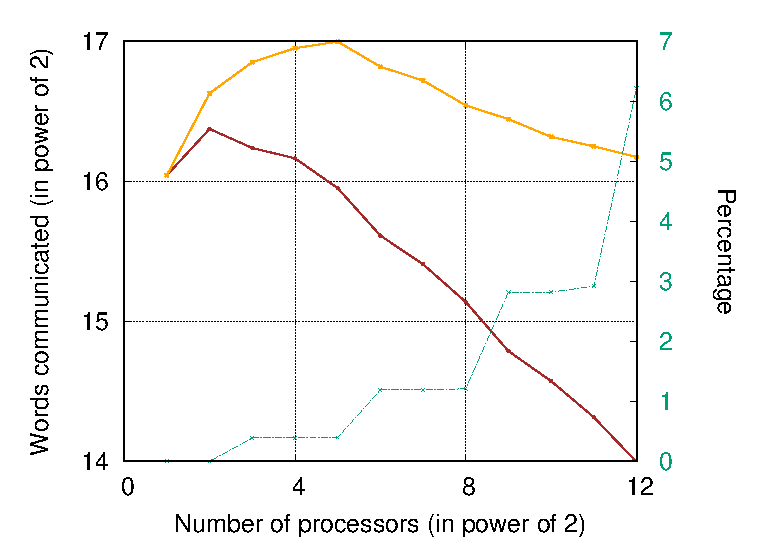
\includegraphics[width=0.415\linewidth]{./plots/AAO-vs-Seq-logscale-comparison-with-comp-12-4.eps}
			}$\quad$
			\subfigure[Input and output tensor dimensions are $13\times13\times13$ and $6\times6\times6$, respectively.]{
				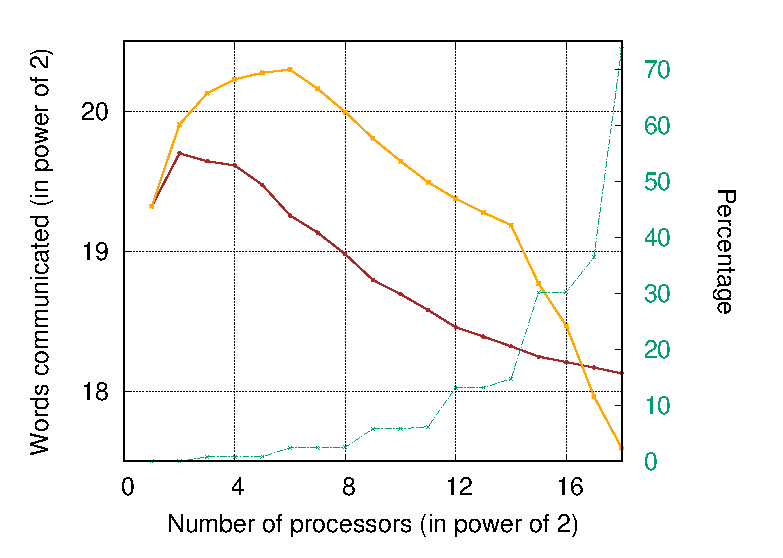
\includegraphics[width=0.415\linewidth]{./plots/AAO-vs-Seq-logscale-comparison-with-comp-13-6.eps}
			}
			\vspace*{-0.135cm}\caption{Comparison of all at once and sequence approaches for two 3-dimensional Multi-TTM computations. $Comp$-$Overhead$ shows the percentage of computational overhead of all at once with respect to the sequence approach.\label{fig:compAllatonceInseq}}
		\end{center}\vspace*{-0.475cm}		
	\end{figure}

	This result also exhibits that neither is better than the other in terms of communication costs for all inputs. It indicates that by combining both of these approaches we can obtain better gains. This encourages us to study how to perform this computation such that the communication is optimal. 
	
	
	
	
	Sequentially truncated HOSVD is another popular method to compute Tucker decomposition~\cite{VVM-SIAM-2012}. After each SVD computation, it performs a single TTM and work on the reduce data for the next SVD computation. Therefore, it performs less computations than the original HOSVD. However when the computational costs of the matrix SVDs are reduced using randomization, costs for both methods are dominated by the Multi-TTM computation. HOSVD is well suited for parallelization as different SVDs can be computed in parallel. It also provides flexibility in the computation of Multi-TTM (see Section~\ref{sec:combinedapproach}). Therefore, we focus on this method to compute Tucker decomposition in the proposal.		
	
	\subsection{State of the art approaches for CP decomposition}
	\label{sec:context:soa:Canonical}
	Computing a CP decomposition involves solving a nonlinear optimization problem to minimize the approximation error. The workhorse method to compute this decomposition uses an alternating least squares (ALS) approach. This works in multiple iterations. Algorithm~\ref{alg:canonicalals} computes a $R$-rank CP decomposition of a $d$-dimensional tensor $\X$ using ALS~\cite{KB-SIAM-2009}. Here $*$ and $\odot$ denote Hadamard and Khatri-Rao products, respectively. Similar to the previous subsection, $X_{(i)}$ represents the $i$th unfolding matrix of $\X$. 
	
	\begin{algorithm}[t]{
			\caption{CP-ALS method to compute CP decomposition\label{alg:canonicalals}}
			\begin{algorithmic}[1]
				\Require input tensor $\X$, desired rank $R$, initial factor matrices $\Mn{A}{1}, \cdots, \Mn{A}{d}$
				\Ensure $\big[\lambda, \Mn{A}{1}, \cdots, \Mn{A}{d}]$ : A rank-R Canonical decomposition of $\X$
				\Repeat
				\For{$i=1 \text{ to } d$}\label{method:canonical:oneiter:start}
				\State $V\gets{\Mn{A}{1}}^\Tra{\Mn{A}{1}}*\cdots*{\Mn{A}{i-1}}^\Tra{\Mn{A}{i-1}}*{\Mn{A}{i+1}}^\Tra{\Mn{A}{i+1}}*\cdots{\Mn{A}{d}}^\Tra{\Mn{A}{d}}$
				\State ${\Mn{A}{i}}\gets X_{(i)} ({\Mn{A}{d}}\odot\cdots\odot{\Mn{A}{i+1}}\odot{\Mn{A}{i-1}}\odot {\Mn{A}{1}})$\label{alg:canonicalals:mttkrp}
				\State ${\Mn{A}{i}}\gets {\Mn{A}{i}}V^\dagger$ \Comment $V^\dagger$ is the pseudo inverse of $V$
				\State $\lambda\gets \text{normalize colums of }{\Mn{A}{i}}$ 
				\EndFor\label{method:canonical:oneiter:end}
				\Until converge or the maximum number of iterations
			\end{algorithmic}
	}\end{algorithm}\vspace*{-0.15cm}
	
	In Line~\ref{alg:canonicalals:mttkrp}, the matricized tensor is multiplied with the Khatri-Rao product and this collective operation is known as the matricized-tensor times Khatri-Rao products (MTTKRP) computation~\cite{LCPSV-IPDPS-2017}. This is the bottleneck computation of the CP-ALS method~\cite{BNR-IPDPS-2018,LCPSV-IPDPS-2017}.
	
	A popular choice to compute MTTKRP is to first calculate the explicit Khatri-Rao products and then apply the matricized tensor in a single matrix multiplication~\cite{BK-SIAM-2008}. Another approach is to work with all the inputs at once without forming an intermediate: 
	$$\Mn{A}{j}_{lr} = \sum_{i_1,\cdots,i_{j-1},i_{j+1},\cdots i_d}\X_{i_1,\cdots,i_{j-1},l,i_{j+1},\cdots i_d}\prod_{k\in{\{1,\cdots,j-1,j+1,\cdots,d\}}}\Mn{A}{k}_{i_k r}.$$
	
	Ballard et al.~\cite{BNR-IPDPS-2018} show that the latter approach significantly reduces communication compared to the former one. We can obtain better gains by combining both of them in a unified manner. This encourages us to look at all possible ways to perform MTTKRP such that the communication is optimal.
	
	
	Another state-of-the-art approach to compute a CP decomposition is based on gradients. MTTKRP is also the bottleneck computation for this approach. Hence, improving the performance of MTTKRP will also accelerate gradient-based approach to compute the decomposition.
	
	
%	\subsection{Technical challenges in combining all at once and sequence approaches}
%	\label{sec:challenges}
	\subsection{Combining all at once and sequence approaches}
	\label{sec:combinedapproach}
	
	As mentioned in Section~\ref{sec:context:soa:Tucker}, in \cite{ABGKR-SIMAX-2024}, we observed that neither approach is better than the other for Multi-TTM with all inputs in terms of communication costs. It motivates us to combine both approaches. There are many ways to perform Multi-TTM computation.  We present some of them below for 3-dimensional cubic input and output tensors.	 
	
%	\begin{align*}
%		\Y&=\seqstart\seqstart\seqstart\X\times_1{\Mn{A}{1}}^\Tra \seqend\times_2{\Mn{A}{2}}^\Tra\seqend\times_3{\Mn{A}{3}}^\Tra\seqend,\\
%		\Y&=\allatoncestart\seqstart\X \times_1 {\Mn{A}{1}}^\Tra \seqend \times_2 {\Mn{A}{2}}^\Tra \times_3 {\Mn{A}{3}}^\Tra \allatonceend,\\
%		\Y &= \seqstart\allatoncestart\X \times_1 {\Mn{A}{1}}^\Tra \times_2 {\Mn{A}{2}}^\Tra\allatonceend \times_3 {\Mn{A}{3}}^\Tra\seqend,\\
%		\Y &= \allatoncestart\X \times_1 {\Mn{A}{1}}^\Tra \times_2 {\Mn{A}{2}}^\Tra \times_3 {\Mn{A}{3}}^\Tra\allatonceend.
%	\end{align*}

	\vspace*{-0.375cm}\begin{align*}
\Y=\seqstart\seqstart\seqstart\X\times_1{\Mn{A}{1}}^\Tra \seqend\times_2{\Mn{A}{2}}^\Tra\seqend\times_3{\Mn{A}{3}}^\Tra\seqend,\quad & \Y=\allatoncestart\seqstart\X \times_1 {\Mn{A}{1}}^\Tra \seqend \times_2 {\Mn{A}{2}}^\Tra \times_3 {\Mn{A}{3}}^\Tra \allatonceend,\\
\Y = \seqstart\allatoncestart\X \times_1 {\Mn{A}{1}}^\Tra \times_2 {\Mn{A}{2}}^\Tra\allatonceend \times_3 {\Mn{A}{3}}^\Tra\seqend,\qquad & \Y = \allatoncestart\X \times_1 {\Mn{A}{1}}^\Tra \times_2 {\Mn{A}{2}}^\Tra \times_3 {\Mn{A}{3}}^\Tra\allatonceend.
\end{align*}\vspace*{-0.35cm}

	Here purple parenthesis indicates that the whole computation inside it will be computed with the all at once approach and blue parenthesis denotes a single TTM computation.  Note that here we follow the order of matrices. Changing the order for the rectangular dimensions may minimize the overall communication. It is also reasonable to first operate only with some matrices and then combine the intermediate results with the remaining computations. Our goal is to find the minimal communication cost of this computation and how it should be performed. 
	

	A preliminary study by the principal investigator shows that a combined approach reduces communication compared to the original ones for some inputs (see Figure~\ref{fig:compCombinedAllatonceseq}). It validates our intuitions and boosts our goal to analyze all possible ways to perform  Multi-TTM computations.



%\sk{insert a good label name for the presented combined approach.}

\begin{figure}[htb]
	\begin{center}
		
\includegraphics[scale=0.12]{./plots/all-at-once-seq-combined-label.png}
	\end{center}
	\vspace*{-1cm}\begin{center}
		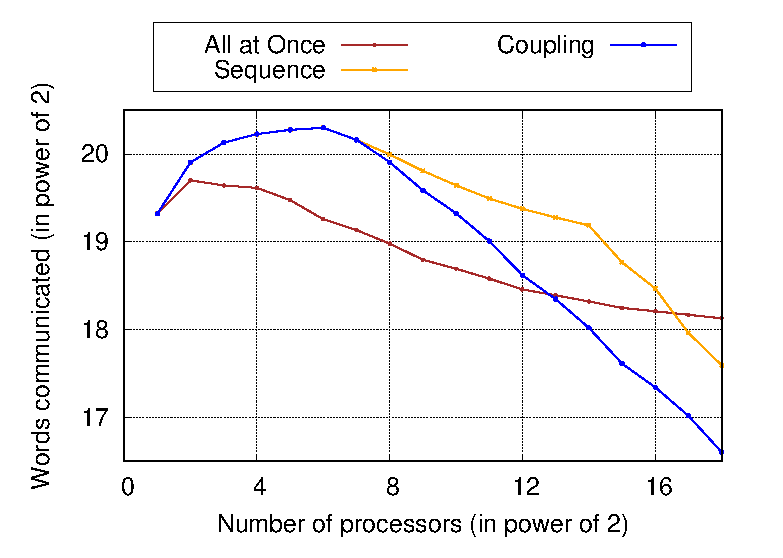
\includegraphics[width=0.45\linewidth]{./plots/AAO-vs-Seq-logscale-comparison-with-coup.eps}
		\vspace*{-0.15cm}\caption{Comparison of all at once and sequence approaches with a combined approach for the second example of Figure~\ref{fig:compAllatonceInseq}. Input and output tensor dimensions are $13\times13\times13$ and $6\times6\times6$, respectively. Here in the combined approach,  all at once approach is applied with first two matrices and then a single TTM is performed with the intermediate  result and the last matrix, $\Y = \seqstart\allatoncestart\X \times_1 {\Mn{A}{1}}^\Tra \times_2 {\Mn{A}{2}}^\Tra\allatonceend \times_3 {\Mn{A}{3}}^\Tra\seqend$. \label{fig:compCombinedAllatonceseq}\vspace*{-0.45cm}}
	\end{center}		
\end{figure}
	

	
	
	
	The amount of operations for Multi-TTM depends on how it is performed, i.e, how factor matrices are operated with the input tensor. Figure~\ref{fig:compAllatonceInseq} shows that the all at once approach increases the amount of operations compared to the sequence approach. It is significantly higher for large number of processors. Therefore, it is also important to study the computation-communication tradeoff for Multi-TTM. 
	
	
%	We will model both communication and computation costs for the Multi-TTM and devise new parallel algorithms such that the overall completion time is minimal. 
	
%	
%	Similar to Multi-TTM, we will study all possible ways to perform $3$ and $4$-dimensional MTTKRP computations. After that, we will generalize our finding and create a dynamic programming based approach to determine how to perform this computation. T
	
	Similar to Multi-TTM, the communication and computation costs of MTTKRP depend on how factor matrices are operated with the original tensor. Therefore it is also important to study communication-computation tradeoff for MTTKRP. We can note that the intermediate Khatri-Rao products may be used between different iterations in Algorithm~\ref{alg:canonicalals}. With 4-dimensional tensors, MTTKRP corresponding to both 1st and 2nd iterations need $\Mn{A}{4}\odot\Mn{A}{3}$. If we store this result in the 1st iteration then it can be reused in the 2nd one. Therefore, it is essential to study tradeoff among communications, computations and reuse of intermediate results for a single iteration (Lines~\ref{method:canonical:oneiter:start}--\ref{method:canonical:oneiter:end}) of CP-ALS method.
	
	
	
	\subsubsection{Challenges and our approaches to tackle them}
	
	As mentioned earlier, the computations and communication costs of Multi-TTM and MTTKRP depend on how we perform them, i.e., how matrices are operated with the input tensor. If we do not select it carefully, their completion times may be very far from the optimal ones. Even when we decide how we want to perform the computations, combining all at once and sequence approaches, using one after the other, in a straightforward way will only work if data distributions of inputs and temporaries between both approaches are compatible. However we can not expect any guarantees with respect to the optimal communication/computation costs. Considering optimal data distributions for only one approach may induce significant data movements for the other approach. Using optimal data distributions for both approaches may not be compatible or require significant data movement during the transition of the approach. Therefore, in order to take benefits of both all at once and sequential approaches, it is important to theoretical study all possible ways to combine them in detail. More precisely, we need to perform the following tasks to design efficient combined approaches for Multi-TTM and MTTKRP:
	
	
%	We need to tackle the following challenges in order to take benefits of both all at once and sequential approaches.
	\begin{itemize}
		\item Analyze communication costs for all possible ways to perform both computations 
		\item Investigate tradeoff among amount of operations, communications and data reuse
		\item Design communication optimal parallel algorithms
%		\item Design and implement parallel HOSVD and CP-ALS methods and test on various datasets
%		\item Analytically determine  arrangement of logical processor grid for better performance
	\end{itemize}
	
	
	We will study all possible ways to perform $3$ and $4$-dimensional Multi-TTM and MTTKRP computations in detail as the number of ways are limited. After that, we will generalize our findings and create a dynamic programming based approach to determine how to perform $d$-dimensional Multi-TTM and MTTKRP computations.
	
	\paragraph{Design optimal algorithms for complete methods}
	As mentioned in the previous subsections, Multi-TTM and MTTKRP are  the bottleneck computations of HOSVD and CP-ALS methods, respectively. After performing detailed study of Multi-TTM and MTTKRP, we will design parallel algorithms such that the overall completion times of HOSVD and CP-ALS are minimal. We will implement our algorithms for homogeneous systems and test them on various datasets. 
	
	In Figures~\ref{fig:compAllatonceInseq} and \ref{fig:compCombinedAllatonceseq}, we used exhaustive search to determine the arrangement of processors that minimizes the cost of each approach. In order to avoid exhaustive search, we plan to determine processor grid dimensions analytically based on the components of communication lower bounds. We will equate communication cost expressions of all matrices/tensors with their corresponding lower bounds and solve them such that all the constraints (with larger terms) are satisfied.
	

	
	
	\subsection{Strategy for parallel algorithms and their implementations}
	
	The HOSVD and CP-ALS methods illustrated in Algorithms~\ref{alg:hosvd} and ~\ref{alg:canonicalals} work with different matrix representations of a tensor. However changing one matrix representation to another results in huge data transfers on distributed memory machines. We plan to directly work with the tensor. We will design our parallel algorithms in a way such that they work with subtensors at each step. This strategy will avoid the need of reshaping a tensor into multiple matrix representations. We will also assume that each input and output are distributed across all nodes in the start and end, respectively.
	
	In the beginning, we plan to implement our parallel algorithms using MPI. All the communications of this implementation would be performed with collectives. This is a simple and popular strategy to minimize communication for many linear algebra kernels on homogeneous systems~\cite{ABK-IPDPS-2016,BKK-TOMS-2020}.
	
	
%	\todo{Clarify how much is expected from the postdoc here.}
	
	As MPI collectives are based on global synchronization, they may not make effective utilization of all the resources. Therefore, later in the project, while working with heterogeneous resources (see Section~\ref{sec:extension:heterogeneoussystem}), we will design our parallel algorithms in task-based structure. This will enable one to run them efficiently with popular runtime systems such as StarPU~\cite{ATNW-CCPE-2011} on modern computing platforms.
	  
	
	
	 
	
	\subsection{Tensor decompositions on heterogeneous systems}
	\label{sec:heterogeneous}
	
	Accelerators such as GPU provide massive computational power at limited cost and energy, therefore they have become a crucial element of many present HPC systems~\cite{top500}. A significant amount of research has been conducted on optimizing sparse MTTKRP, TTM and tensor decompositions on heterogeneous systems~\cite{NLSVS-IPDPS-2019,LWSD-CLUSTER-2017,parti}. 
	
%	,NHCLTSRPC-ICS-2022
	
	There is limited work on performing dense tensor decompositions on heterogeneous systems. Choi et al.~\cite{CLC-SC-2018} implemented the dense Tucker decomposition method on GPUs and achieved significant speedup over CPU-only implementations. Bin et al.~\cite{BKL-SENSORS-2020} proposed a GPU based framework to accelerate tensor decompositions for image sensor data. Li et al.~\cite{li2020atucker} proposed a framework to handle diversities of the input tensors for Tucker decomposition on CPUs and GPUs and showed that it outperforms the existing approaches. These works implemented the existing algorithms for GPUs and applied different types of optimizations to improve the performance. Their approaches perform well for the considered tensors, however they lack provable guarantees for communication/computation/overall costs. The SCATE project addresses this concern.
	
		
	\subsubsection{Extending our framework for heterogeneous systems}
	\label{sec:extension:heterogeneoussystem}
	In the beginning of this project, we will mainly focus on designing optimal algorithms for homogeneous systems. After that, we plan to extend our framework for heterogeneous systems with CPUs and GPUs. We will mainly consider the following three types of systems:
	
	\begin{figure}[htb]
		\begin{center}
			\subfigure[A single node with one CPU and one GPU.\label{system:onecpugpu}]
			{\begin{tikzpicture}[scale=0.67, every node/.style={transform shape}]
				\tikzstyle{cpunode}=[draw=black, minimum height=16mm, minimum width=16mm, fill=none, text=black, below]
				\tikzstyle{gpunode}=[draw=black, minimum height=12mm, minimum width=12mm, fill=none, text=black]
				
				\tikzstyle{memorynode}=[draw=black, minimum height=4mm, minimum width=4mm, fill=none, text=black]
				
				\node (t0) at (0,0) [cpunode] {$CPU$}; 
				\node (t1) at (0,-4) [gpunode] {};
				
				\node (t1G) at (t1.mid) [below] {$GPU$};
				\node (td0)  at (t0.mid) [below=0.275cm,memorynode,scale=0.6] {$Memory$};
				\node (td1)  at (t1.north) [below=0.15cm,memorynode,scale=0.5] {$Memory$};
				\draw [<->, line width=1.5, orange] (td0) -- (td1);
				\path (-2.25,0) -- (2.58,0);
				\end{tikzpicture}}$\quad$
			\subfigure[A single node with one CPU and multiple GPUs.\label{system:onecpumultiplegpus}]
			{\begin{tikzpicture}[scale=0.67, every node/.style={transform shape}]
				\tikzstyle{cpunode}=[draw=black, minimum height=16mm, minimum width=16mm, fill=none, text=black, below]
				\tikzstyle{gpunode}=[draw=black, minimum height=12mm, minimum width=12mm, fill=none, text=black]
				
				\tikzstyle{memorynode}=[draw=black, minimum height=4mm, minimum width=4mm, fill=none, text=black]
				
				
				
				\node (t0) at (0,0) [cpunode] {$CPU$}; 
				\node (t1) at (-2,-4) [gpunode] {};
				\node (t2) at (2,-4) [gpunode] {};
				
				\node (t1G) at (t1.mid) [below] {$GPU$};
				\node (t2G) at (t2.mid) [below] {$GPU$};
				
				\node (td0)  at (t0.mid) [below=0.275cm,memorynode,scale=0.6] {$Memory$};
				\node (td1)  at (t1.north) [below=0.15cm,memorynode,scale=0.5] {$Memory$};
				\node (td2)  at (t2.north) [below=0.15cm,memorynode,scale=0.5] {$Memory$};
				
				\draw [<->, line width=1.5, red] (td1) -- (td2);
				\draw [<->, line width=1.5, orange] (td0) -- (td1);
				\draw [<->, line width=1.5, orange] (td0) -- (td2);
				
				\end{tikzpicture}}$\qquad$
			\subfigure[Multiple nodes where each node has one CPU and atleast one GPU.\label{system:gen}]
			{\begin{tikzpicture}[scale=0.67, every node/.style={transform shape}]
				\tikzstyle{cpunode}=[draw=black, minimum height=16mm, minimum width=16mm, fill=none, text=black, below]
				\tikzstyle{gpunode}=[draw=black, minimum height=12mm, minimum width=12mm, fill=none, text=black]
				
				\tikzstyle{memorynode}=[draw=black, minimum height=4mm, minimum width=4mm, fill=none, text=black]
				
				
				
				\node (t0) at (0,0) [cpunode] {$CPU$}; 
				\node (t1) at (-2,-4) [gpunode] {};
				\node (t2) at (2,-4) [gpunode] {};
				
				\node (t1G) at (t1.mid) [below] {$GPU$};
				\node (t2G) at (t2.mid) [below] {$GPU$};
				
				\node (td0)  at (t0.mid) [below=0.275cm,memorynode,scale=0.6] {$Memory$};
				\node (td1)  at (t1.north) [below=0.15cm,memorynode,scale=0.5] {$Memory$};
				\node (td2)  at (t2.north) [below=0.15cm,memorynode,scale=0.5] {$Memory$};
				
				\draw [<->, line width=1.5, red] (td1) -- (td2);
				\draw [<->, line width=1.5, orange] (td0) -- (td1);
				\draw [<->, line width=1.5, orange] (td0) -- (td2);
				
				
				\node (t20) at (6,0) [cpunode] {$CPU$};
				\node (t21) at (4,-4) [gpunode] {};
				\node (t22) at (8,-4) [gpunode] {}; 
				
				\node (t21G) at (t21.mid) [below] {$GPU$};
				\node (t22G) at (t22.mid) [below] {$GPU$};
				
				\node (td20)  at (t20.mid) [below=0.275cm,memorynode,scale=0.6] {$Memory$};
				\node (td21)  at (t21.north) [below=0.15cm,memorynode,scale=0.5] {$Memory$};
				\node (td22)  at (t22.north) [below=0.15cm,memorynode,scale=0.5] {$Memory$};
				\draw [<->, line width=1.5, purple] (td0) -- (td20);
				
				\draw [<->, line width=1.5, red] (td21) -- (td22);
				\draw [<->, line width=1.5, orange] (td20) -- (td21);
				\draw [<->, line width=1.5, orange] (td20) -- (td22);
				\end{tikzpicture}}
			\vspace*{-0.05cm}\caption{Different types of heterogeneous systems.\label{fig:heterogeneousSystems}}
		\end{center}\vspace*{-0.25cm}		
	\end{figure}
	
	Usually there are many processing units attached to a particular memory module. However to simplify the model, we view them as a single big computing unit.
	The project will first study different metrics to express the communication and complete costs on the above types of systems. After that we will focus on the first type of system. We will study tradeoff among computations, communications and data reuse for both tensor decompositions and design algorithms which achieve optimal completion times. Next, we will expand our framework for the other two types of heterogeneous systems. Implementation of the proposed algorithms for heterogeneous systems is out of scope of this project. We will submit another proposal to hire an engineer for that work.
	
	\subsection{Objectives}
	\label{sec:context:obj}
	
	The goal of the SCATE project is to devise Tucker and CP decomposition algorithms which scale well on the modern computing systems. Recent work~\cite{ABGKR-SIMAX-2024} made by the principal investigator (PI) of this project started to address the bottleneck computation of Tucker decomposition and obtained encouraging preliminary results. The complete parallel algorithms for these decompositions with provable guarantees on their performances are still missing. The main focus of the SCATE project is to address this aspect.
	
%	\newpage
	%%\sk{May be something on the state of the art approaches}
	
	The project first studies tradeoff among computations, communications and data reuse for popular tensor decomposition methods and proposes new parallel algorithms whose completion times are optimal for homogeneous systems. After that, the proposed algorithms will be implemented and tested with various datasets on the distributed machines available at ENS Lyon. We will also examine scalability of our algorithms on more than 5,000 cores and/or 512 nodes of \href{https://www.genci.fr/en/our-computers}{GENCI (Grand Equipement de Calcul Intensif)}, which includes the supercomputers from CEA and CNRS.

	
	
	Significant amount of performance is produced by accelerators for the present HPC systems, including many at GENCI. So developing only homogeneous algorithms ignores too much computation power and may result in poor efficiency on heterogeneous systems. The project does address this concern and extends the proposed algorithms for heterogeneous systems with CPUs and GPUs.
	
	

	

	\subsection{Datasets}
	\label{sec:context:datasets}
	We will first assess performance of all our algorithms on synthetic data. After that, we will use the datasets of~\cite{BKK-TOMS-2020} to evaluate our parallel Multi-TTM and HOSVD algorithms.
	\begin{itemize}
		\item SP: This is a $500 \times 500 \times 500 \times 11 \times 400$ tensor data. It is obtained from a combustion simulation. It corresponds to a $500 \times 500 \times 500$ spatial cubic grid for $11$ variables over $400$ time steps. The size of the entire dataset is 4.4 TB. 
		\item JICF: This is a $500 \times 2080 \times 1500 \times 18 \times 10$ tensor data. It is obtained from a jet in cross-flow simulation. It corresponds to a $500 \times 2080 \times 1500$ spatial grid with $18$ variables over $10$ time steps. The size of the entire dataset is 6.7 TB.
	\end{itemize}
	
	\noindent We will use the Mouse dataset of~\cite{EHBKMP-TOMS-2021} to evaluate our parallel MTTKRP and CP-ALS algorithms.
	\begin{itemize}
		\item Mouse dataset: This is a 3-dimensional dataset that corresponds to images of a mouse's brain over time and over a sequence of identical trials. Each entry of the tensor represents a measure of calcium fluorescence in a particular pixel during a time step of a single trial. Each image has dimension $1040\times 1392$ and the number of time steps across $25$ trials is $69$. By flattening the pixel dimensions, it results in a $1446680 \times 69 \times 25$ tensor. 
	\end{itemize}
	We are already in touch with the authors of the mentioned papers and they are ready to share data with us.
%%	As mentioned earlier, tensors are used to store data in several domains. 
	We will also contact people from different fields such as astrophysics and neuroscience who work with high-dimensional dense data and request them to share their datasets with us. We will evaluate our algorithms on them as well.
	
	
	\medskip
	
	\noindent\url{http://frostt.io/tensors} stores several sparse tensors obtained from real applications. Thanks to this, a significant amount of research has been conducted on sparse tensor computations in the last 7 years. However we have observed relatively less work on dense tensor computations. The SCATE project, with the help of other researchers from tensor community, plans to setup a public repository to store dense tensors of real applications. We will seek support from Inria/CNRS to host this repository.
%%	We will use Inria cloud storage for this. 
	We will add all the used real-world tensors in the project to that repository. We will also add code snippets of real applications that generate dense tensors, such as correlation functions. We believe this repository will help researchers to work more on dense tensor computations. 
	
%%	\noindent\url{http://frostt.io/tensors} stores several sparse tensor datasets obtained from real applications. Thanks to this, a significant amount of research has been conducted on sparse tensor computations in the last 6 years. However we have observed relatively less work on dense tensor computations. We believe that the accessibility of large real-world tensors is one of the main reasons for this. The SCATE project, with the help of other researchers from tensor community, plans to setup a public repository to store dense tensor data of real applications. We will use Inria cloud storage for this repository. We will add all the used real-world tensors in this project to that repository. We will also add code snippets of real applications that generate dense tensors, such as correlation functions. 
%%	 -- high order correlation functions, stochastic PDEs, for example. 
	
	\subsection{Risk management}
	\label{sec:context:risk}
	
	There are two main risks with this project, but we believe they are not critical to its success.
	
	The first risk is that our algorithms may not improve the state of the art for all settings. As mentioned in Section~\ref{sec:combinedapproach}, in our preliminary study we observed that a simple combined approach is better than individual sequence and all at once approaches for some inputs. This indicates that by unifying all possible ways to combine both approaches we will be equal or better than the state of the art for all settings.
%%	Therefore we believe that our algorithms will significantly outperform all existing ones.
	
	The second risk is that some of our algorithms may perform more communication than the proposed lower bounds. We aim to obtain all parameters of an algorithm from different terms of the corresponding lower bound. However this may not always be possible as it requires to match multiple terms with reasonable values. In such scenarios we aim to exactly match the larger terms and bound the increase in the smaller terms by the larger terms. This approach will provide the parameters of our algorithms with which they attain the lower bounds within a constant factor.
	

\newpage



	\section{Project organisation and implementation}
	\label{sec:org}
	 We present the PI and his team in Section~\ref{sec:org:team} and the tasks and the work packages of the project in Section~\ref{sec:org:projstructure}. In Sections~\ref{sec:org:wp:homo} and~\ref{sec:org:wp:hetero}, we describe the contents of each work package, before discussing the provisional schedule in Section~\ref{sec:org:taskschedule}. In Section~\ref{sec:org:costs}, we detail the cost of the project. In Section~\ref{sec:org:growth}, we present the impact of the project on the PI's growth and the team development around the topic.

%%	Demonstrate how this project is contributing to the empowerment of a young researcher and the team development around the theme.
	
	
	\begin{table}[htb]
		\begin{center}
			\scalebox{0.9}{
				\begin{tabular}{lllr}
					\hline
					\rowcolor{orange}
					Name & Position &  Contribution & Involvement \\
					\hline \hline
					Suraj Kumar & ISFP Inria &  Principal investigator & 36 PM\\ \hline
					Loris Marchal & DR2 CNRS, HdR & Will work on WPB1--WPB4 & 6 PM\\ \hline
					Bora Uçar & DR2 CNRS, HdR & Will work on WPA2--WPA4& 6 PM\\ \hline
					PhD Student     & \textbf{Funded by ANR} & WPA1--WPA4 & 36 PM \\ \hline
					Postdoctoral Researcher & \textbf{Funded by ANR} & WPB1--WPB5 & 24 PM \\ \hline
					Research Intern &  \textbf{Funded by ANR} & WPA5 & 6 PM\\ \hline
					Research Intern &  \textbf{Funded by ANR} & WPA6 & 6 PM\\
					\bottomrule
			\end{tabular}}
		\end{center}
		\vspace*{-0.35cm}\caption{Human resources.}
		\label{tab:human}
	\end{table}
	
	\vspace*{-0.35cm}\subsection{The principal investigator and his team}
	\label{sec:org:team}
	Suraj Kumar holds an Inria Starting Faculty Position (ISFP) since October 2022 in the ROMA Inria team, which is hosted at École Normale Supérieure de Lyon (ENS Lyon). He is an expert in tensor computations, communication avoiding algorithms and efficient utilization of resources on heterogeneous systems. He defended his thesis in April 2017 on Scheduling of Dense Linear Algebra Kernels on Heterogeneous Resources. After that, he joined Ericsson Research, India as an engineer and worked on the use of remote GPUs in cloud. He was a post-doctorate researcher at Pacific Northwest National Laboratory, USA from May 2018 to October 2019. He worked there on \href{https://www.exascaleproject.org/research-project/nwchemex}{NWChemEx} project, whose main goal was to run molecular simulations efficiently on exascale computers. He also worked at Inria Paris from November 2019 to September 2022 as a postdoctoral researcher on the design of parallel and communication optimal algorithms for Multi-TTM computations and tensor-train decompositions. He has collaborated with over 25 researchers all over the world. In particular he has an active collaboration with Grey Ballard of Wake Forest University, USA, who is an expert in the design of communication-efficient algorithms, that will be beneficial to the implementation of the project. The PI will dedicate 75\% of his research time on this project.
	
	
	
	The project will be pursued in the ROMA Inria team at ENS Lyon. It will include Loris Marchal (DR2, CNRS, HdR) and Bora Uçar (DR2, CNRS, HdR). Table~\ref{tab:human} summarizes the implication of each member of the project, including people hired by this ANR project.
	
		
	Bora Uçar is an expert in the design of efficient algorithms for sparse tensor computations. He will help the PI in supervising the PhD student and is expected to be a PhD co-advisor. He will be greatly involved in \textbf{WPA3} and \textbf{WPA4} and help in \textbf{WPA2} to study reuse with dimension tree approach.
	
	
	Loris Marchal is an expert in memory aware computations and designing efficient scheduling algorithms for heterogeneous systems. He will help the PI to supervise the postdoctoral researcher. He will be involved in \textbf{WPB1}--\textbf{WPB4} of \textbf{Task B}.
	
	The major recruitments of the SCATE project are the PhD student and the postdoctoral researcher. The PhD student is expected to join the project from the beginning and will focus on design and implementation of scalable tensor decomposition algorithms for homogeneous systems. The postdoctoral researcher is expected to be hired for 24 months, starting at the middle of the project. He/She will extend the proposed algorithms for heterogeneous systems. He/She will also help the PI to advise the PhD student.
	
	The project also includes two master-level research interns. They are expected to join the project towards the end of 3rd year and will wok on the algorithms developed by the PhD student. The first intern will study numerical guarantees of the proposed algorithms and the second intern will explore how to apply mixed precision arithmetic to further improve the algorithms.
			
	\vspace*{-0.15cm}\subsection{Project structure}
	\label{sec:org:projstructure}
	The SCATE project has two tasks. \textbf{Task A} focuses on homogeneous systems and \textbf{Task B} targets heterogeneous systems. \textbf{Task A} is further subdivided into six main work packages.
	\begin{itemize}
		\item \textbf{WPA1} obtains communication lower bounds for the bottleneck computations (Multi-TTM and MTTKRP) of Tucker and CP decomposition methods.
		\item \textbf{WPA2} analyzes tradeoff among computations, communications and data reuse for the complete tensor decomposition methods.
		\item \textbf{WPA3} designs new parallel algorithms which achieve optimal completion times.
		\item \textbf{WPA4} implements the proposed algorithms for distributed memory homogeneous systems and validates the performance improvement on the machines available at ENS Lyon and GENCI.
		\item \textbf{WPA5} studies the numerical robustness of the proposed algorithms.
		\item \textbf{WPA6} explores how to apply mixed precision arithmetic to further improve our algorithms.
	\end{itemize}
	
	
	Similarly, \textbf{Task B} is further subdivided into five main work packages.
	\begin{itemize}
		\item \textbf{WPB1} studies different metrics to express communication and overall costs on heterogeneous systems with CPUs and GPUs.
		\item \textbf{WPB2} focuses on a single simple heterogeneous node. It obtains communication lower bounds for the bottleneck computations of both decompositions and studies tradeoff among computations, communications and data reuse for the complete methods.
		\item \textbf{WPB3} devises new parallel algorithms, by taking advantage of the knowledge obtained in \textbf{WPB2}, that achieve optimal completion times on a single simple heterogeneous node.
		\item \textbf{WPB4} extends our frameworks (\textbf{WPB2} and \textbf{WPB3}) to general heterogeneous systems.
		\item \textbf{WPB5} is exploratory in nature and will be performed in the last $4$ months of the project. It incorporates practical information of the systems such as efficiency on CPU and GPU, maximum saturation of each bandwidth link in our algorithms. It also investigates energy costs of our algorithms and proposes strategies to make them energy optimal.
	\end{itemize}
	
	
	
	
	%%We will begin with \textbf{Task A}. Our framework for \textbf{WPA1} and \textbf{WPA2} will be ready within a year. We will also have good understanding of structure of computations and communications for the decomposition algorithms by then. We plan to extend our framework for heterogeneous systems at this point and start \textbf{Task B}.

	
	
	
	The work packages \textbf{WPA1} -- \textbf{WPA6} address homogeneous systems and \textbf{WPB1} -- \textbf{WPB5} target heterogeneous systems.
	\vspace*{-0.15cm}\subsection{Description of the work packages for homogeneous systems}
	\label{sec:org:wp:homo}
	
	
	\subsubsection{\textbf{WPA1}: Bottleneck computations of both decompositions}
	\vspace*{-0.385cm}\begin{table}[H]
		\begin{tabular}{lll}
			\hline
			\cellcolor{blue2}
			Members involved & Suraj Kumar& PhD Student \\
			\hline
			\cellcolor{orange2}
			Involvement      & 4 PM            & 8 PM \\
			\hline
		\end{tabular}
	\end{table}\vspace*{-0.25cm}
	
%	\newpage
	\subtask{Subtask A1.1: Multi-TTM minimum communication costs}
	\begin{itemize}[leftmargin=-1pt]
		\item[] \goal To obtain communication lower bounds for Multi-TTM.
%	\end{itemize}
%	\begin{itemize}[leftmargin=-1pt]
%		\item[] \goal To obtain communication lower bounds for Multi-TTM.
		\item[] \dwp A key question would be to understand what is the minimum amount of data transfer is required to perform Multi-TTM in parallel. As mentioned in Section~\ref{sec:combinedapproach}, there are multiple ways to perform this computation. We will look at all possible ways (as these are limited) to perform 3 and 4-dimensional computations. For each way, we will represent the amount of access of every input/output on a processor with one variable and construct an optimization problem whose objective function is convex and all the constraints can be expressed with quasiconvex functions. After that we will analytically solve the optimization problem with the help of Lagrange multipliers methods and Karush-Kuhn-Tucker (KKT) conditions, similar to the ones used in~\cite{ABGKR-SIMAX-2024}.
		
		
		It is sometimes hard to directly compare analytical solutions of several approaches. Therefore we will graphically plot them to have better understanding of how different factors influence the amount of data transfers. Following that we will generalize the analytical solutions for higher dimensions. 
		
		Finally we will create a dynamic programming based approach to determine the minimum amount of data transfers for a Multi-TTM computation and how it should be performed. The code for this approach will be made available under a free software license.
		
		\item[] \deliverables T0+6: A description of the dynamic programming based approach to determine the minimum communication cost of Multi-TTM (report)
%%		\newline
%%		T0+6: An implementation of the approach (software)
	\end{itemize}
	
	\subtask{Subtask A1.2: MTTKRP minimum communication costs}
	\begin{itemize}[leftmargin=-1pt]
		\item[] \goal To obtain communication lower bounds for MTTKRP.
		\item[] \dwp Similar to the previous subtask, we will analyze data transfer costs of all possible ways to perform MTTKRP involving 3 and 4-dimensional tensors. After that, we will generalize our observations for the computations involving higher dimensions and create a dynamic programming based approach to determine the minimum communication cost.
		\item[] \deliverables T0+9: A description of the dynamic programming based approach to determine how MTTKRP should be performed to minimize the communication cost (report)\newline
		T0+9: An implementation of the approach for Multi-TTM and MTTKRP (software)	
	\end{itemize}
	
	\subsubsection{\textbf{WPA2}: Tradeoff among communications, computations and reuse}
	\begin{table}[H]
		\begin{tabular}{llll}
			\hline
			\cellcolor{blue2}
			Members involved & Suraj Kumar& Bora Uçar & PhD Student \\
			\hline
			\cellcolor{orange2}
			Involvement      & 6 PM            & 1 PM & 10 PM \\
			\hline
		\end{tabular}
	\end{table}
	\subtask{Subtask A2.1: Cost modeling for Multi-TTM and MTTKRP}
	\begin{itemize}[leftmargin=-1pt]
		\item[] \goal To analyze amount of operations and communication costs for Multi-TTM and MTTKRP. 
		\item[] \dwp As mentioned earlier, the amount of operations and data transfers for both Multi-TTM and MTTKRP depend on how they are performed. This subtask intends to take advantage of \textbf{WPA1} and add the amount of operations in dynamic programming approach. Here we note that it is possible that once the data transfer costs among processors are determined then rearranging local computations may minimize the amount of operations. This is what we observed for Multi-TTM with the all at once approach in our preliminary study~\cite{ABGKR-SIMAX-2024}. We will express the overall cost as $\alpha\cdot$ amount of operations + $\beta\cdot$ amount of data transfers. Here $\alpha$ and $\beta$ represent the weight of the processing power (arithmetic cost per unit operation) and transfer capability (transfer cost per unit data ) of a system. We will analyze this cost for various practical values of $\alpha$ and $\beta$.
		\item[] \deliverables T0+14: A description of the overall cost models for Multi-TTM and MTTKRP (report)
%%		\newline
%%		T0+14: Include this model in the existing implementation of dynamic programming based approach (software)
	\end{itemize}
	\subtask{Subtask A2.2: Cost modeling for HOSVD and CP-ALS methods}
	\begin{itemize}[leftmargin=-1pt]
		\item[] \goal To study comprise among computations, communications and data reuse for both methods. 
		\item[] \dwp The previous subtask analyzes costs of the bottleneck computations of both methods. This subtask focuses on the full methods. For HOSVD, we will determine the cost of each computation and then sum them to obtain the overall cost. This will be an expression in terms of amount of operations and data transfers. This expression may not be very precise when two significant computations require different data distributions. However for HOSVD, when we employ randomized SVDs to compute factor matrices then the overall cost is dominated by Multi-TTM.
		
		A single iteration of the CP-ALS method performs $d$ MTTKRPs. As mentioned in Section~\ref{sec:combinedapproach}, some intermediate computations between MTTKRPs can be reused. This will reduce the total amount of operations. Recently, Kaya and Uçar~\cite{KU-SISC-2018} used dimension trees to exploit reuse among all the MTTKRPs of a single iteration. This subtask intends to apply dimension tree approach to reduce the computations in all possible ways to perform MTTKRPs and then determine the overall cost of a single iteration in terms of amount of operations and data transfers.
		\item[] \deliverables T0+18: A description of the overall costs of HOSVD and CP-ALS methods (report)\newline
		T0+18: An implementation of the dynamic programming based approach to express the overall costs for both methods (software)
	\end{itemize}
	
	\subsubsection{\textbf{WPA3}: Design new parallel algorithms}
	\vspace*{-0.375cm}\begin{table}[H]
		\begin{tabular}{llll}
			\hline
			\cellcolor{blue2}
			Members involved & Suraj Kumar& Bora Uçar & PhD Student \\
			\hline
			\cellcolor{orange2}
			Involvement      & 2 PM            & 2 PM & 7 PM \\
			\hline
		\end{tabular}
	\end{table}\vspace*{-0.25cm}
	%%\subtask{Subtask}
	\begin{itemize}[leftmargin=-1pt]
		\item[] \goal Develop new parallel algorithms for both methods.
		\item[] \dwp The previous task \textbf{WPA2} specifies how different computations should be performed in both methods. Based on this information, \textbf{WPA3} designs parallel algorithm. Here the aim is that computation/communication cost corresponding to a particular variable (matrix or tensor) should be same as in \textbf{WPA2}. It may require to logically view the processors in a multi-dimensional grid. The previous work packages determine minimum communication costs by solving constrained optimization problems and have used only one variable for each input/output. An input/output usually has more than one dimension. Therefore we need to interpret the solutions of constrained optimization problems in multiple dimensions. This requires us to look at all the variables in a solution at once and determine how to partition each dimension to devise an algorithm. It may not always result in reasonable partitions. Recently we show that determining processor grid dimensions from the communication lower bounds of Multi-TTM in the all at once approach may require some extra adaptation~\cite{ABGKR-SIMAX-2024}. However we observe that we can bound overall communication cost of any variable in terms of that of the largest tensor. We plan to prove theoretical guarantees of the new algorithms in similar ways.
		
		If the communication cost of the algorithms is very far from the theoretical cost, we will spend more time on \textbf{WPA2} to understand what extra constraints we need to include. 
		\item[] \deliverables T0+24: A description of the parallel HOSVD algorithm and its optimality proof (report)
		T0+27: A description of the parallel CP-ALS algorithm and its optimality proof (report) 
	\end{itemize}
	
	\vspace*{-0.635cm}\subsubsection{\textbf{WPA4}: Experimental evaluation of the proposed algorithms}
	\vspace*{-0.385cm}\begin{table}[H]
		\begin{tabular}{llll}
			\hline
			\cellcolor{blue2}
			Members involved & Suraj Kumar& Bora Uçar & PhD Student \\
			\hline
			\cellcolor{orange2}
			Involvement      & 3 PM            & 3 PM & 11 PM \\
			\hline
		\end{tabular}
	\end{table}\vspace*{-0.25cm}
	\subtask{Subtask A4.1: Implementation of the algorithms}
	\begin{itemize}[leftmargin=-1pt]
		\item[] \goal To implement the proposed algorithms and run them on GENCI machines.
		\item[] \dwp This subtasks implements the proposed algorithms in \textbf{WPA3} for both HOSVD and CP-ALS methods. Initially it will use machines available at ENS Lyon for debugging and execution. It will verify the scalability of the proposed algorithms by running them on GENCI machines for several datasets including the ones mentioned in Section~\ref{sec:context:datasets}. The code will be made available under a free software license.
		\item[] \deliverables T0 +36: Implementation of the proposed algorithms for both methods (software)	
	\end{itemize}
		\subtask{Subtask A4.2: Storing real dense tensor datasets}
	\begin{itemize}[leftmargin=-1pt]
		\item[] \goal To setup a repository to store dense real-world tensors.
		\item[] \dwp This subtask aims to create a public repository and to store all the used real-world tensors in the project to that repository. We will also request other researchers to store\linebreak similar tensors there. It will serve as a benchmark and will help the whole tensor community.
		\item[] \deliverables T0 +42: A repository to store dense tensor data of real applications (repository)	
	\end{itemize}

	\subsubsection{\textbf{WPA5}: Numerical robustness of the proposed algorithms}
	\vspace*{-0.385cm}\begin{table}[H]
		\begin{tabular}{lll}
			\hline
			\cellcolor{blue2}
			Members involved & Suraj Kumar& Research Intern \\
			\hline
			\cellcolor{orange2}
			Involvement      & 1 PM            & 6 PM \\
			\hline
		\end{tabular}
	\end{table}\vspace*{-0.25cm}
	%%\subtask{Subtask}
	\begin{itemize}[leftmargin=-1pt]
		\item[] \goal To study numerical robustness of the algorithms developed in \textbf{WPA3}.
		\item[] \dwp Computations may be arranged differently than the conventional ways in the previous work packages. This will also change the numerical robustness of the algorithms. \textbf{WPA5} aims to study and compare numerical properties of our algorithms with the state of the art. 
		\item[] \deliverables
		T0+36: Numerical guarantees of the proposed algorithms (report)
	\end{itemize}
	\subsubsection{\textbf{WPA6}: Applying mixed precision arithmetic}
	\vspace*{-0.385cm}\begin{table}[H]
		\begin{tabular}{lll}
			\hline
			\cellcolor{blue2}
			Members involved & Suraj Kumar& Research Intern \\
			\hline
			\cellcolor{orange2}
			Involvement      & 2 PM            & 6 PM \\
			\hline
		\end{tabular}
	\end{table}\vspace*{-0.25cm}
	%%\subtask{Subtask}
	\begin{itemize}[leftmargin=-1pt]
		\item[] \goal To apply mixed precision arithmetic to further improve our algorithms.
		\item[] \dwp Performing mixed precision arithmetic is a promising direction to improve performance of many scientific computations. \textbf{WPA6} explores how to apply mixed precision arithmetic to further improve our algorithms.
		\item[] \deliverables T0+39: Improved algorithms for both methods (report)
	\end{itemize}
	
	
	\subsection{Description of the work packages for heterogeneous systems}
	\label{sec:org:wp:hetero}	
	%%Starting time: T0+24	
	\subsubsection{\textbf{WPB1}: Metrics to express costs}
	\vspace*{-0.385cm}\begin{table}[H]
		\begin{tabular}{llll}
			\hline
			\cellcolor{blue2}
			Members involved & Suraj Kumar& Loris Marchal & Postdoctoral Researcher \\
			\hline
			\cellcolor{orange2}
			Involvement      & 2 PM            & 1 PM & 2 PM \\
			\hline
		\end{tabular}
	\end{table}\vspace*{-0.25cm}
\newpage
	%%\subtask{Subtask B1.1: }
	\begin{itemize}[leftmargin=-1pt]
		\item[] \goal To study different parameters to formulate costs on heterogeneous systems.
		\item[] \dwp This subtask analyzes different hardware characteristics such as processing and transfer capabilities, network topology in detail for all the three types of systems of Figure~\ref{fig:heterogeneousSystems}. The main purpose of this subtask is to propose simplified models for communication, computation and overall costs. 
		\item[] \deliverables T0 +26: A description of the cost models for heterogeneous systems (report) 
	\end{itemize}
	
	\subsubsection{\textbf{WPB2}: Costs on a single simple heterogeneous node}
	\vspace*{-0.385cm}\begin{table}[H]
		\begin{tabular}{llll}
			\hline
			\cellcolor{blue2}
			Members involved & Suraj Kumar& Loris Marchal & Postdoctoral Researcher \\
			\hline
			\cellcolor{orange2}
			Involvement      & 4 PM            & 1 PM & 7 PM \\
			\hline
		\end{tabular}
	\end{table}\vspace*{-0.25cm}
	\begin{itemize}[leftmargin=-1pt]
		\item[] \goal To develop minimum cost expressions for both decomposition methods. 
		\item[] \dwp \textbf{WPB2} focuses on Figure~\ref{system:onecpugpu} type of system (a single simple heterogeneous node). It will first obtain expressions for Multi-TTM and MTTKRP computations. Due to heterogeneity, we need to solve optimization problems with more variables and constraints to determine the minimum communication costs. If all the constraints can not be expressed with quasiconvex function then we may not obtain analytical solutions. In such cases we plan to employ optimization softwares to solve them.
		Following that, we plan to study tradeoff among computations, communication and reuse for both HOSVD and CP-ALS methods, and derive the minimum cost expressions in terms of amount of computations and communications. 
		\item[] \deliverables
		T0+29: A description of the cost expressions for Multi-TTM and MTTKRP (report)\newline
		T0+ 33: A description of the cost expression for the complete methods (report)
	\end{itemize}
	
	\subsubsection{\textbf{WPB3}: Devise new algorithms}
	\vspace*{-0.385cm}\begin{table}[H]
		\begin{tabular}{llll}
			\hline
			\cellcolor{blue2}
			Members involved & Suraj Kumar& Loris Marchal & Postdoctoral Researcher \\
			\hline
			\cellcolor{orange2}
			Involvement      & 2 PM            & 2 PM & 3 PM \\
			\hline
		\end{tabular}
	\end{table}\vspace*{-0.25cm}
	%%\subtask{Subtask B1.1: }
	\begin{itemize}[leftmargin=-1pt]
		\item[] \goal To design new algorithms for both methods. 
		\item[] \dwp This task intends to take advantage of the knowledge obtained in \textbf{WPB2} and design new algorithms whose completion times are optimal for a single simple heterogeneous node.
		\item[] \deliverables T0 +36: A description of the complete algorithms for HOSVD and CP-ALS methods (report)
	\end{itemize}
	
	\subsubsection{\textbf{WPB4}: Algorithms for more than one GPU}
	\vspace*{-0.35cm}\begin{table}[H]
		\begin{tabular}{llll}
			\hline
			\cellcolor{blue2}
			Members involved & Suraj Kumar& Loris Marchal & Postdoctoral Researcher \\
			\hline
			\cellcolor{orange2}
			Involvement      & 6 PM            & 2 PM & 8 PM \\
			\hline
		\end{tabular}
	\end{table}\vspace*{-0.05cm}
	\subtask{Subtask B4.1: Devise algorithms for a single heterogeneous node.}
	\begin{itemize}[leftmargin=-1pt]
		\item[] \goal To extend \textbf{WPB2} and \textbf{WPB3} for more than one GPU of a single node.
		\item[] \dwp This subtask focuses on Figure~\ref{system:onecpumultiplegpus} type of system. It expands the results of the previous two work packages to a node with multiple GPUs. It will develop complete algorithms for HOSVD and CP-ALS methods that achieve optimal completion times.
		\item[] \deliverables
		T0 +41: A description of the complete algorithms for both methods (report)
	\end{itemize}
	\subtask{Subtask B4.2: Devise algorithms for multiple heterogeneous nodes.}
	\begin{itemize}[leftmargin=-1pt]
		\item[] \goal To extend \textbf{WPB2} and \textbf{WPB3} for general heterogeneous systems.
		\item[] \dwp This subtask focuses on Figure~\ref{system:gen} type of system, which is very common in HPC. Multiple GPUs are connected to each node and nodes are connected among themselves. Similar to the previous subtask, it will develop complete algorithms for both methods that achieve optimal completion times on multiple heterogeneous nodes.
		\item[] \deliverables T0 +44: A description of the complete algorithms for HOSVD and CP-ALS methods (report) 
	\end{itemize}
	
		\subsubsection{\textbf{WPB5}: Incorporate empirical information}
\vspace*{-0.385cm}\begin{table}[H]
	\begin{tabular}{lll}
		\hline
		\cellcolor{blue2}
		Members involved & Suraj Kumar & Postdoctoral Researcher \\
		\hline
		\cellcolor{orange2}
		Involvement      & 4 PM     & 4 PM \\
		\hline
	\end{tabular}
\end{table}\vspace*{-0.25cm}
%%\subtask{Subtask B1.1: }
\begin{itemize}[leftmargin=-1pt]
	\item[] \goal To include factual system information in our algorithms.
	\item[] \dwp This work package is exploratory in nature. It intends to include more empirical information, such as efficiency of a processing unit, saturation level of bandwidth links, missing link between two nodes, in our algorithms. It will also investigate energy costs of our algorithms and propose strategies to make them energy optimal.
	\item[] \deliverables T0 +48: Energy analysis of our algorithms (report) 
\end{itemize}



\subsection{Task schedule and deliverables}
\label{sec:org:taskschedule}
We present a tentative schedule of the work packages and their subtasks in Table~\ref{tab:gantt} and summarize the different deliverables in Table~\ref{tab:deliverables}.




\subsection{Resource management}
\label{sec:org:costs}
\subsubsection*{Costs supported by ANR proposal}
\paragraph{Staff} A PhD student (36 months), a postdoctoral researcher (24 months) and two research interns (master-level, 6 months) will be hired for the project. 

\paragraph{Mission, traveling} The project also includes funding to participate to international/national conferences/workshops. The traveling costs for these are evaluated as follows:
\begin{itemize}
	\item Attending 3 international conferences for the PI, 2 for the PhD student, 2 for the postdoctoral researcher during 4 years. Cost: (3+2+2) $\times $ 2.5k\euro $=$ 17.5k\euro.
	\item Attending 4 workshops/conferences in France for the PI, 3 for the PhD student and 2 for the postdoctoral researcher during 4 years. Cost: (4+3+2) $\times$ 1k\euro $=$ 9k\euro.
\end{itemize}
We plan to organize a two-day workshop on tensor computations in Lyon at the beginning of Year 3, whose cost (food and breaks) will be partly supported by ANR (20 people). Cost: 2500\euro.

\paragraph{Inward billing} Laptops for the PhD student and the postdoctoral researcher. Cost: 2$\times$2.5k\euro $=$ 5k\euro.







	
	%%\newcommand{\oc}{\cellcolor{orange1}}
	%%\newcommand{\br}{\cellcolor{blue2}{\ding{45}}}% delivrable rapport
	%%\newcommand{\bs}{\cellcolor{blue2}{\ding{171}}}% delivrable soft
	%%\newcommand{\bsr}{\cellcolor{blue2}{\ding{45}\ding{171}}}% delivrable soft
	%%\newcommand{\gc}{\cellcolor{green}{\ding{171}}}% delivrable soft
	%%\newcommand{\re}{\cellcolor{gray}{}}% delivrable soft
	
	
	
	\newcommand{\oc}{\cellcolor{orange1}}
	\newcommand{\br}{\cellcolor{orange1}{\ding{45}}}% delivrable rapport
	\newcommand{\bs}{\cellcolor{orange1}{\ding{171}}}% delivrable soft
	\newcommand{\bsr}{\cellcolor{orange1}{\ding{45}\ding{171}}}% delivrable soft
	\newcommand{\gc}{\cellcolor{green}{\ding{171}}}% delivrable soft
	\newcommand{\re}{\cellcolor{gray}{}}% delivrable soft
	\newcommand{\orepo}{\cellcolor{orange1}{\ding{95}}}% delivrable rapport
	
	
	
	\begin{table}
		\begin{center}
			\scalebox{0.925}{
				\begin{tabular}{c|c|c|c|c|c|c|c|c|c|c|c|c|c|c|c|c|c|}
					\cline{3-18}%
					\multicolumn{2}{l|}{}&
					\multicolumn{4}{c|}{Year 1}&
					\multicolumn{4}{c|}{Year 2}&
					\multicolumn{4}{c|}{Year 3}&
					\multicolumn{4}{c|}{Year 4}
					\\
					\cline{3-18}%
					\multicolumn{2}{c|}{}              &   3 &   6 &   9 &  12 &  15 &  18 &  21 &  24 &  27 &  30 &  33 &  36 &  39 &  42 &  45 &  48 \\ \hline \cline{3-18}
					\multirow{2}{*}{WPA1} &
					\multicolumn{1}{|r||}{Subtask A1.1} & \oc & \br &     &     &     &     &     &     &     &     &     &     &     &     &     &     \\ \cline{2-18} &
					\multicolumn{1}{|r||}{Subtask A1.2} &  & \oc & \bsr &     &     &     &     &     &     &     &     &     &     &     &     &     \\ \hline \hline
					
					
					\multirow{2}{*}{WPA2} &
					\multicolumn{1}{|r||}{Subtask A2.1} &  &  & \oc    &\oc     &\br     &     &     &     &     &     &     &     &     &     &     &     \\ \cline{2-18} &
					\multicolumn{1}{|r||}{Subtask A2.2} &  &  & & \oc & \oc    & \bsr    &     &     &     &     &     &     &     &     &     &     \\ \hline \hline
					
					\multirow{1}{*}{WPA3} &
					\multicolumn{1}{|r||}{} &     &     &     &     &     &     &  \oc   & \br    &  \br   &     &     &     &     &     &     &  \\ \hline \hline
					
					
					\multirow{2}{*}{WPA4} &
					\multicolumn{1}{|r||}{Subtask A4.1} &     &     &     &     &     &     &     &     &  \oc   &  \oc   &  \oc   & \bs    &     &     &     & \\ \cline{2-18} &
					\multicolumn{1}{|r||}{Subtask A4.2} &     &     &     &     &     &     &     &     &     &     &  \oc   & \oc    & \oc     & \orepo    &     & \\ \hline \hline
					
					\multirow{1}{*}{WPA5} &
					\multicolumn{1}{|r||}{} &     &     &     &     &     &     &     &     &     &     &  \oc   & \br    &     &     &     &  \\ \hline \hline
					
					\multirow{1}{*}{WPA6} &
					\multicolumn{1}{|r||}{} &     &     &     &     &     &     &     &     &     &     &     & \oc    &  \br   &     &     &  \\ \hline \hline
					
					\multirow{1}{*}{WPB1} &
					\multicolumn{1}{|r||}{} &     &     &     &     &     &     &     &     & \br    &     &     &     &     &     &     &  \\ \hline \hline
					
					\multirow{1}{*}{WPB2} &
					\multicolumn{1}{|r||}{} &     &     &     &     &     &     &     &     & \oc    & \br    &  \br   &     &     &     &     &  \\ \hline \hline
					
					\multirow{1}{*}{WPB3} &
					\multicolumn{1}{|r||}{} &     &     &     &     &     &     &     &     &     &     &     &  \br   &     &     &     &  \\ \hline \hline
					
					\multirow{2}{*}{WPB4} &
					\multicolumn{1}{|r||}{Subtask B4.1} &  &  &     &     &     &     &     &     &     &     &     &     & \oc    &  \br   &     &     \\ \cline{2-18} &
					\multicolumn{1}{|r||}{Subtask B4.2} &  &  & &  &     &     &     &     &     &     &     &     &     & \oc    & \br    &     \\ \hline \hline
					
					\multirow{1}{*}{WPB5} &
					\multicolumn{1}{|r||}{} &     &     &     &     &     &     &     &     &     &     &     &     &     &     &   \oc  & \br \\ \hline \hline
					
					
					\multicolumn{2}{c|}{PhD Student}                 & \re & \re & \re & \re & \re & \re & \re & \re & \re & \re & \multicolumn{2}{c}{\re Writing} &     &  &     &    \\ \hline
					\multicolumn{2}{c|}{Postdoctoral Researcher}          &     &     &     &     &     &     &     &     &\re  & \re & \re & \re & \re & \re & \re   & \re   \\ \hline
					\multicolumn{2}{c|}{Research Intern}            &  &  &     &     &     &     &     &     &     &  \re   &  \re   &     &     &     &     &      \\ \hline
					\multicolumn{2}{c|}{Research Intern}            &  &  &     &     &     &     &     &     &     &     &  \re   &  \re   &     &     &     &      \\ \hline
				\end{tabular}%
			}
			\newline\newline
			\scalebox{0.975}{
			\begin{tabular}{rlcccccc}
				\oc & Working on task  &&\ding{45} $\;$ Report deliverable &&\ding{95} $\;$ Repository deliverable && \ding{171} $\;$ Code deliverable  
			\end{tabular}
			}
		\end{center}
		\vspace*{-0.25cm}\caption{Tentative task schedule.}
		\label{tab:gantt}
	\end{table}
	
	%%\ding{45} report
	%%\ding{171} software
	
	
	\begin{table}
		\begin{center}
			\scalebox{0.925}{
				\begin{tabular}{|c|c|c|c|}
					\rowcolor{blue2}
					Work package &  Subtask & Deliverable & Date (month) \\ \hline
					
					\multirow{2}{*}{WPA1} & Subtask A1.1 & Report & T0+6\\
					&  Subtask A1.2 & Report+code & T0+9\\ \hline
					
					\multirow{2}{*}{WPA2} & Subtask A2.1 & Report & T0+14\\
					&  Subtask A2.2 & Report+code & T0+18\\ \hline
					
					WPA3 &  & Report & T0+24, T0+27\\ 
					&	& Workshop & T0+27 \\ \hline
					
					\multirow{2}{*}{WPA4} & Subtask A4.1 & Code & T0+36\\
					&Subtask A4.2& Repository & T0+42\\ \hline
					WPA5 & & Report & T0+36\\ \hline
					WPA6 & & Report & T0+39\\ \hline
					
					
					WPB1 & & Report & T0+26\\ \hline
					WPB2 & & Report & T0+29, T0+33\\ \hline
					WPB3 & & Report & T0+36\\ \hline
					
					\multirow{2}{*}{WPB4} & Subtask B4.1 & Report & T0+41\\
					&  Subtask B4.2 & Report & T0+44\\ \hline
					
					WPB5 & & Report & T0+48\\ \hline
			\end{tabular}}
		\end{center}
		\vspace*{-0.25cm}\caption{Summary of deliverables.}
		\label{tab:deliverables}
	\end{table}
	
	



\begin{table}[h]
	\begin{center}
		\begin{tabular}{p{3.8cm}p{8.25cm}r}
			\toprule
			%				\multicolumn{1}{l}{}&& Inria Lyon \\\midrule
			\multirow{3}{3.8cm}{Staff expenses}  & PhD student &   120k\euro \\\cline{2-3}
			& Postdoctoral researcher  &100k\euro \\ \cline{2-3}
			& 2 Research interns  & 6.6k\euro \\\hline
			\multicolumn{2}{p{7cm}}{Inward billing (2 laptops)}    &    5k\euro \\\hline
			\multirow{3}{3.8cm}{General and administrative costs \& other
				 expenses}  & Travel costs (international and local missions)  &  26.5k\euro \\\cline{2-3}
			& Partial cost to organize a workshop  &  2.5k\euro \\\cline{2-3}
			& Administrative management costs& 37 787\euro \\\midrule
			\multicolumn{2}{l}{\bf Requested} &\multicolumn{1}{r}{298 387\euro} \\
			\bottomrule
		\end{tabular}
	\end{center}
	\vspace*{-0.45cm}\caption{Estimated cost of the project.\vspace*{-0.25cm}}
	\label{tab:costs}
\end{table}


	\subsubsection*{Costs not supported by ANR proposal}
	\begin{itemize}[leftmargin=-1pt]
		\item[] \textbf{Experimental resources} We will initially use the machines available at ENS Lyon for our experiments. We also plan to ask compute-hours on GENCI to test scalability of our proposed algorithms.
		\item[] \textbf{Additional visits} We will look for additional funding from Inria/CNRS for a three month scientific visit for the PhD student to launch new collaborations (for instance around the Cyclops~\cite{SMHD-IPDPS-2013}/TuckerMPI~\cite{BKK-TOMS-2020}/ Deinsum~\cite{ZKBSH-SC-2022} library team) and to broaden his future perspectives.		
		\item[] \textbf{Hiring of an engineer} This project (\textbf{Task B}) will develop provable algorithms for heterogeneous systems. We will submit another proposal to hire an engineer who will work on the implementation of these algorithms. The engineer will also work on combining our and TuckerMPI softwares (and other popular ones provided we manage to get good support from their contributors) in a unified framework.	
	\end{itemize}
%	\paragraph{Experimental resources} We will initially use the machines available at ENS Lyon for our experiments. We also plan to ask compute-hours on GENCI to test scalability of our proposed algorithms.
%	
%	%%\paragraph{Additional travels and workshop} We will ask for additional funding from the ENS Lyon for a three months internship of the PhD student at Wake Forest University, Winston-Salem, North Carolina, USA. 
%	
%	
%	
%	
%	\paragraph{Additional visits} We will look for additional funding from Inria/CNRS for a three month scientific visit for the PhD student to launch new collaborations (for instance around the Cyclops~\cite{SMHD-IPDPS-2013}/TuckerMPI~\cite{BKK-TOMS-2020}/Deinsum~\cite{ZKBSH-SC-2022} library team) and to broaden his future perspectives.
%	
%%	We will also seek additional funding to organize another workshop at the end of $4$th Year.
%	
%	\paragraph{Hiring of an engineer} This project (\textbf{Task B}) will develop provable algorithms for heterogeneous systems. We will submit another proposal to hire an engineer who will work on the implementation of these algorithms. The engineer will also work on combining our and TuckerMPI softwares (and other popular ones provided we manage to get good support from their contributors) in a unified framework.
	
%%	• Project contribution to the coordinator’s empowerment and team development
%%Demonstrate the project contribution to the young researcher’s empowerment and team development.sec:org:growth
	\subsection{Growth of the PI and team development}
	\label{sec:org:growth}
	Tensors are used in several domains. Therefore acceptance of this proposal certainly will improve the visibility of the PI in various research communities. We expect to publish the obtained results in major conferences/journals of the field. We also plan to present our work on relevant conferences, symposiums and workshops. These will enhance the visibility of the team and allow us to engage with other researchers and start new collaborations.

	
	
%%	This will also broaden the perspective of the temporary employees and help them to achieve their next career goals.
%%	Tensors are used in several domains. Therefore acceptance of this proposal certainly will improve the visibility of the PI in various research communities. We expect to publish the obtained results of this project to the major venues (conferences/journals) of the field. This will enhance the visibility of the team. We plan to attend relevant conferences, symposiums and workshops and present our work there. This will allow us to discuss with other researchers and start new collaborations. This will also broaden the perspective of the temporary employees and help them to achieve their next career goals. 
	
	Nowadays multi-dimensional data is ubiquitous. However its analysis is challenging. Working actively on the design of parallel tensor decomposition algorithms will definitely attract attentions of people who work on data analysis. There are many research labs in Lyon such as \href{https://www.crnl.fr/}{CRNL} who analyze biological data. Collaborating with them will allow us to gain insight of realistic data and may help us to propose data specific decompositions. This will be useful for long term collaborations and enable us to submit interdisciplinary research and development proposals in future.
	
	As mentioned earlier, we plan to organize a workshop on tensor computations in Lyon at the beginning of third year. We plan to invite researchers from all over the Europe. Furthermore we plan to organize a minisymposium on tensor decompositions at SIAM Conference on Computational Science and Engineering (CSE25). These will allow us to have fruitful discussions and establish close collaborations.
	
	
	

	\section{Project impact and consequences}
	\label{sec:impact}
%%	Scientific impact and possible impact in economic, social and cultural fields	
	\subsection*{Impact of the project}
	The parallel algorithms developed within the project will substantially improve the capabilities to perform data analytics on modern computing systems. This will lead to a strong impact in domains that deal with large amount of multi-dimensional data. For example, medical research, scientific simulations, data mining, computer vision and astrophysics, to name a few. The large amount of data transfers is one of the main bottlenecks for big data analytics and extreme scale visualization~\cite{DOE-Report-2014}. The project employs communication avoidance strategies to design parallel algorithms and implement them for homogeneous systems. This should allow scientists to solve significantly larger problems and explore new ideas. The communication avoidance strategy also reduces energy consumption that helps to minimize carbon footprint.
	
	The public repository to store dense tensors of real applications will be very helpful for the whole tensor community. It will allow them to test their tensor algorithms on realistic data. We expect that it will become a classical benchmark, like SuiteSparse for sparse matrices.
	
%%	 serve as a benchmark.
	
%%Strategy for the dissemination and exploitation of the results; promotion of scientific, technical and industrial culture
	
	\subsection*{Dissemination and exploitation of the results}
	
	First, a website including all materials and information (progress, reports, deliverables, papers, slides, software) related to the project will be available to the public and kept up-to-date.
	
	
	We expect to publish the obtained results in major scientific conferences (SC, IPDPS, SPAA, EuroPar) and journals (SIMAX, SISC, TOMS, TPDS). Preliminary results such as implementation prototypes, simulation results of cost models will be presented in poster sessions and demos co-located with major scientific conferences. SIAM conferences and workshops are very valuable events and most of them are without published proceeding. We also plan to present our work there. The algorithms that will be developed in this project will be freely available. We will publish the code under a free license. We will provide documentation and keep it up-to-date. This will create opportunities for outside people to use our code and engage with us.
	
%	offers  \emph{Data-aware algorithms for matrix and tensor computations} course for the 2nd year master students at ENS Lyon.
	
	The PI also plans to offer a course on multi-dimensional data analysis for the 2nd year master students at ENS Lyon. All materials of this courses will be available on the PI's personal webpage.
	
	
%%	The lectures of this course will be recorded and will be available on the PI's personal webpage.

	
	{\footnotesize
		\bibliographystyle{IEEEtranS}
		\bibliography{scate}
	}
	
\end{document}
